\documentclass[]{book}
\usepackage{lmodern}
\usepackage{amssymb,amsmath}
\usepackage{ifxetex,ifluatex}
\usepackage{fixltx2e} % provides \textsubscript
\ifnum 0\ifxetex 1\fi\ifluatex 1\fi=0 % if pdftex
  \usepackage[T1]{fontenc}
  \usepackage[utf8]{inputenc}
\else % if luatex or xelatex
  \ifxetex
    \usepackage{mathspec}
  \else
    \usepackage{fontspec}
  \fi
  \defaultfontfeatures{Ligatures=TeX,Scale=MatchLowercase}
\fi
% use upquote if available, for straight quotes in verbatim environments
\IfFileExists{upquote.sty}{\usepackage{upquote}}{}
% use microtype if available
\IfFileExists{microtype.sty}{%
\usepackage{microtype}
\UseMicrotypeSet[protrusion]{basicmath} % disable protrusion for tt fonts
}{}
\usepackage[margin=1in]{geometry}
\usepackage{hyperref}
\hypersetup{unicode=true,
            pdftitle={A Reading Guide to Intuitive Biostatistics},
            pdfauthor={Nathan Brouwer},
            pdfborder={0 0 0},
            breaklinks=true}
\urlstyle{same}  % don't use monospace font for urls
\usepackage{natbib}
\bibliographystyle{apalike}
\usepackage{color}
\usepackage{fancyvrb}
\newcommand{\VerbBar}{|}
\newcommand{\VERB}{\Verb[commandchars=\\\{\}]}
\DefineVerbatimEnvironment{Highlighting}{Verbatim}{commandchars=\\\{\}}
% Add ',fontsize=\small' for more characters per line
\usepackage{framed}
\definecolor{shadecolor}{RGB}{248,248,248}
\newenvironment{Shaded}{\begin{snugshade}}{\end{snugshade}}
\newcommand{\KeywordTok}[1]{\textcolor[rgb]{0.13,0.29,0.53}{\textbf{#1}}}
\newcommand{\DataTypeTok}[1]{\textcolor[rgb]{0.13,0.29,0.53}{#1}}
\newcommand{\DecValTok}[1]{\textcolor[rgb]{0.00,0.00,0.81}{#1}}
\newcommand{\BaseNTok}[1]{\textcolor[rgb]{0.00,0.00,0.81}{#1}}
\newcommand{\FloatTok}[1]{\textcolor[rgb]{0.00,0.00,0.81}{#1}}
\newcommand{\ConstantTok}[1]{\textcolor[rgb]{0.00,0.00,0.00}{#1}}
\newcommand{\CharTok}[1]{\textcolor[rgb]{0.31,0.60,0.02}{#1}}
\newcommand{\SpecialCharTok}[1]{\textcolor[rgb]{0.00,0.00,0.00}{#1}}
\newcommand{\StringTok}[1]{\textcolor[rgb]{0.31,0.60,0.02}{#1}}
\newcommand{\VerbatimStringTok}[1]{\textcolor[rgb]{0.31,0.60,0.02}{#1}}
\newcommand{\SpecialStringTok}[1]{\textcolor[rgb]{0.31,0.60,0.02}{#1}}
\newcommand{\ImportTok}[1]{#1}
\newcommand{\CommentTok}[1]{\textcolor[rgb]{0.56,0.35,0.01}{\textit{#1}}}
\newcommand{\DocumentationTok}[1]{\textcolor[rgb]{0.56,0.35,0.01}{\textbf{\textit{#1}}}}
\newcommand{\AnnotationTok}[1]{\textcolor[rgb]{0.56,0.35,0.01}{\textbf{\textit{#1}}}}
\newcommand{\CommentVarTok}[1]{\textcolor[rgb]{0.56,0.35,0.01}{\textbf{\textit{#1}}}}
\newcommand{\OtherTok}[1]{\textcolor[rgb]{0.56,0.35,0.01}{#1}}
\newcommand{\FunctionTok}[1]{\textcolor[rgb]{0.00,0.00,0.00}{#1}}
\newcommand{\VariableTok}[1]{\textcolor[rgb]{0.00,0.00,0.00}{#1}}
\newcommand{\ControlFlowTok}[1]{\textcolor[rgb]{0.13,0.29,0.53}{\textbf{#1}}}
\newcommand{\OperatorTok}[1]{\textcolor[rgb]{0.81,0.36,0.00}{\textbf{#1}}}
\newcommand{\BuiltInTok}[1]{#1}
\newcommand{\ExtensionTok}[1]{#1}
\newcommand{\PreprocessorTok}[1]{\textcolor[rgb]{0.56,0.35,0.01}{\textit{#1}}}
\newcommand{\AttributeTok}[1]{\textcolor[rgb]{0.77,0.63,0.00}{#1}}
\newcommand{\RegionMarkerTok}[1]{#1}
\newcommand{\InformationTok}[1]{\textcolor[rgb]{0.56,0.35,0.01}{\textbf{\textit{#1}}}}
\newcommand{\WarningTok}[1]{\textcolor[rgb]{0.56,0.35,0.01}{\textbf{\textit{#1}}}}
\newcommand{\AlertTok}[1]{\textcolor[rgb]{0.94,0.16,0.16}{#1}}
\newcommand{\ErrorTok}[1]{\textcolor[rgb]{0.64,0.00,0.00}{\textbf{#1}}}
\newcommand{\NormalTok}[1]{#1}
\usepackage{longtable,booktabs}
\usepackage{graphicx,grffile}
\makeatletter
\def\maxwidth{\ifdim\Gin@nat@width>\linewidth\linewidth\else\Gin@nat@width\fi}
\def\maxheight{\ifdim\Gin@nat@height>\textheight\textheight\else\Gin@nat@height\fi}
\makeatother
% Scale images if necessary, so that they will not overflow the page
% margins by default, and it is still possible to overwrite the defaults
% using explicit options in \includegraphics[width, height, ...]{}
\setkeys{Gin}{width=\maxwidth,height=\maxheight,keepaspectratio}
\IfFileExists{parskip.sty}{%
\usepackage{parskip}
}{% else
\setlength{\parindent}{0pt}
\setlength{\parskip}{6pt plus 2pt minus 1pt}
}
\setlength{\emergencystretch}{3em}  % prevent overfull lines
\providecommand{\tightlist}{%
  \setlength{\itemsep}{0pt}\setlength{\parskip}{0pt}}
\setcounter{secnumdepth}{5}
% Redefines (sub)paragraphs to behave more like sections
\ifx\paragraph\undefined\else
\let\oldparagraph\paragraph
\renewcommand{\paragraph}[1]{\oldparagraph{#1}\mbox{}}
\fi
\ifx\subparagraph\undefined\else
\let\oldsubparagraph\subparagraph
\renewcommand{\subparagraph}[1]{\oldsubparagraph{#1}\mbox{}}
\fi

%%% Use protect on footnotes to avoid problems with footnotes in titles
\let\rmarkdownfootnote\footnote%
\def\footnote{\protect\rmarkdownfootnote}

%%% Change title format to be more compact
\usepackage{titling}

% Create subtitle command for use in maketitle
\newcommand{\subtitle}[1]{
  \posttitle{
    \begin{center}\large#1\end{center}
    }
}

\setlength{\droptitle}{-2em}

  \title{A Reading Guide to Intuitive Biostatistics}
    \pretitle{\vspace{\droptitle}\centering\huge}
  \posttitle{\par}
    \author{Nathan Brouwer}
    \preauthor{\centering\large\emph}
  \postauthor{\par}
      \predate{\centering\large\emph}
  \postdate{\par}
    \date{2018-09-07}

\usepackage{booktabs}
\usepackage{amsthm}
\makeatletter
\def\thm@space@setup{%
  \thm@preskip=8pt plus 2pt minus 4pt
  \thm@postskip=\thm@preskip
}
\makeatother
\usepackage{booktabs}
\usepackage{longtable}
\usepackage{array}
\usepackage{multirow}
\usepackage[table]{xcolor}
\usepackage{wrapfig}
\usepackage{float}
\usepackage{colortbl}
\usepackage{pdflscape}
\usepackage{tabu}
\usepackage{threeparttable}
\usepackage{threeparttablex}
\usepackage[normalem]{ulem}
\usepackage{makecell}

\usepackage{amsthm}
\newtheorem{theorem}{Theorem}[chapter]
\newtheorem{lemma}{Lemma}[chapter]
\theoremstyle{definition}
\newtheorem{definition}{Definition}[chapter]
\newtheorem{corollary}{Corollary}[chapter]
\newtheorem{proposition}{Proposition}[chapter]
\theoremstyle{definition}
\newtheorem{example}{Example}[chapter]
\theoremstyle{definition}
\newtheorem{exercise}{Exercise}[chapter]
\theoremstyle{remark}
\newtheorem*{remark}{Remark}
\newtheorem*{solution}{Solution}
\begin{document}
\maketitle

{
\setcounter{tocdepth}{1}
\tableofcontents
}
\chapter*{Preface}\label{preface}
\addcontentsline{toc}{chapter}{Preface}

This is a reading guide to Harvey Motulsky's
\href{http://www.intuitivebiostatistics.com/}{Intuitive Biostatistics: A
Nonmathematical Guide to Statistical Thinking}, 4th edition. More
information about the book can be found at the
\href{http://www.intuitivebiostatistics.com/}{book's website},
\url{http://www.intuitivebiostatistics.com/}, and it can be purchased
from
\href{https://www.amazon.com/Intuitive-Biostatistics-Nonmathematical-Statistical-Thinking/dp/0190643560/ref=asap_bc?ie=UTF8}{Amazon.com}.
Motulsky is the CEO and Founder of
\href{https://www.graphpad.com/}{GraphPad}, a user-friendly statistical
software popular in some branches of the life sciences.

\emph{Intutitive Biostatistics} is a fabulous book for researchers that
need to understand or do basic statistics and either need a concise
primer on the key issues and/or are turned off by the equations
underlying the statistical methods. Instead of using math to explain
statistical methods, Motulsky focuses on written explanations,
real-world examples, and novel graphing approaches. An excellent aspect
of this book is that it unpacks common misunderstandings that
researchers have, such as how to interpret p-values (Chapter 17), and
signposts bad practices that must be avoided (like p-hacking). Again,
this is done by focusing on intuition, not math. Motulsky also presents
best practices in plotting, data presentation, and data reporting,
emphasizing the key aspect of adequate and accurate presentation of
results.

This reading guide serves several purposes:

\begin{itemize}
\tightlist
\item
  Highlight the parts of the book I focus on in my teaching (and so will
  be on any tests!)
\item
  Provide additional complementary examples
\item
  Indicate extensions or alternatives
\item
  Provide citations and links to resources for follow-up
\item
  Indicate where others (including myself, though I am not a trained
  statistician) might disagree with Motulsky
\end{itemize}

Each part of the reading guide is essentially an outline of each chapter
with commentary as needed. In some cases I have written a brief initial
commentary to put the chapter in context. I will often indicate the
Excel or R functions related to methods or calculations; for a fuller
treatment see my other guide \emph{An R Companion to Motulsky's}
Intuitive Biostatistics. At the end of each chapter are typically
references, a list of R and Excel functions needed to carry out the
analyses in the book, and study questions to consider.

My most important notes and comments are generally in \textbf{bold} or
bulleted. When I've riffed on an idea and its not necessarily key I've
usually put in in a block quote, like the one below:

\begin{quote}
For example, sometimes I've written about a section, and my text is
almost as long as the original section!
\end{quote}

This is a work in progress and many sections are not yet annotated; feel
free to contact me with suggestions or corrections.

Nathan Brouwer
\href{mailto:brouwern@gmail.com}{\nolinkurl{brouwern@gmail.com}}

\chapter{\texorpdfstring{``Statistics \& Probablity Are Not
Intuitive''}{Statistics \& Probablity Are Not Intuitive}}\label{ch1}

\section*{Commentary}\label{commentary}
\addcontentsline{toc}{section}{Commentary}

In this introductory chapter Motulsky sketches out some major reasons
why people struggle with statistics and probability. This chapter
assumpes some basic familiarity with statistical ideas. Sometimes this
chapter is a bit terse - its meant to highlight key ideas, not fully
discuss or demonstate them.

\section*{Vocabulary}\label{vocabulary}
\addcontentsline{toc}{section}{Vocabulary}

\subsection*{Motulsky vocab}\label{motulsky-vocab}
\addcontentsline{toc}{subsection}{Motulsky vocab}

\begin{itemize}
\tightlist
\item
  sample
\item
  population
\item
  Bayesian
\item
  multiple comparisons
\item
  regression to the mean
\end{itemize}

\subsection*{Additional vocab}\label{additional-vocab}
\addcontentsline{toc}{subsection}{Additional vocab}

\begin{itemize}
\tightlist
\item
  Bayes theorem
\item
  pre-registration
\item
  exploratory analyses
\end{itemize}

\subsection*{Key functions}\label{key-functions}
\addcontentsline{toc}{subsection}{Key functions}

None

\section*{Chapter Notes}\label{chapter-notes}
\addcontentsline{toc}{section}{Chapter Notes}

\section{We Tend to Jump to
Conclusions}\label{we-tend-to-jump-to-conclusions}

\begin{quote}
Motulsky uses the phrase ``\textbf{generalize from a sample to a
population}'' without defining what this means. In general, this means
to look at some subset of the world - either something experienced in
real life or generated using a scientific study - and conclude that what
was seen in the subset occurs elsewhere. In the example he uses, his
daughter experienced meeting doctors, and they all were male, so she
generalized to the rest of the world that all doctors must be male.
While this example is trivial, anytime we generalize from sample to
population (or from a part to the whole) we run the risk that our sample
is biased. It could be biased becauase we didn't take a good sample,
such as relying just on personal experiencce. Or it could be a
rigorously collected scientific sample, but still be non-representative.
What if he wanted to prove his daughter wrong and so randomly selected
10 doctor's offices for a web search and looked up who the senior
physician is. If he happend to find my doctor's office, he'd see that
its a women, Dr.~Cathy Lamb. However, it is possible that he could look
up 10 doctor's and they could all still be male.
\end{quote}

\section{We Tend to Be Overconfident}\label{we-tend-to-be-overconfident}

\section{We see Patterns in Random
Data}\label{we-see-patterns-in-random-data}

\section{We don't realize that coincidences are
common}\label{we-dont-realize-that-coincidences-are-common}

He doesn't use the specific term, but he is alluding to the concept of
\textbf{hindsight bias}.

\section{We don't expect variability to depend on sample
size}\label{we-dont-expect-variability-to-depend-on-sample-size}

Motulsky cites a paper by Andrew Gelman here, one of the most thought
provoking - though sometimes just provoking -- statistics bloggers of
the last decade. He blogs regularly at
\href{http://andrewgelman.com/}{Statistical Modeling, Causal Inference,
and Social Science} and writes non-technical pieces for a number of
outlets, including
\href{http://www.slate.com/authors.andrew_gelman.html}{Slate}. He is
also prominent Bayesian.

\section{We Have Incorrect Intuitive Feelings About
Probability}\label{we-have-incorrect-intuitive-feelings-about-probability}

\section{We Find it Hard to Combine
Probabilities}\label{we-find-it-hard-to-combine-probabilities}

\section{(We Avoid Thinking About Ambiguous
Situations)}\label{we-avoid-thinking-about-ambiguous-situations}

(This section appear in previous versions; I am not sure where/if it
occurs in the 4th edition)

\section{We Don't Do Bayesian Calculations
Intuitively}\label{we-dont-do-bayesian-calculations-intuitively}

\begin{quote}
Motulsky doesn't define \textbf{Bayesian} here, though its not central
to what he's talking about. In this example, ``Bayesian calculations''
refers to a particular type of probability calculation using
\textbf{Bayes Rule}. His example is a classic example of how probability
calculations are used for diagnostic testing.
\end{quote}

\begin{quote}
More generally, ``Bayesian''" refers to a particular way to use the
mathematics of probability to make inference. All mathematicians agree
on the basic rules of probability calculations. In contrast, when it
comes to using the math of probablity to make inference from a sample to
a population - that is, to do statistics - there is a huge rift between
\textbf{Frequentists} and \textbf{Bayesians}.
\end{quote}

\section{We are Fooled By Multiple
Comparisons}\label{we-are-fooled-by-multiple-comparisons}

The study on astroglogical signs here is a great paper intended to ``To
illustrate how multiple hypotheses testing can produce associations with
no clinical plausibility'' (Austin et al 2006, Abstract). ``Multiple
hypotheses testing'' means the same thing as ``multiple comparisons.''
As Motulsky indicates, if you test multiple hypotheses or make multiple
comparisons between things, sooner or later you'll find a strong
association. This is why it important to make specific hypotheses prior
to the beginning of a study - ideally even publically
\textbf{pre-registering} them - and properly indicate which analyses
were defined in advance and which are \textbf{exploratory analyses}.

\textbf{Multiple Comparisons} is a big topic that Motulsky doesn't go
into detail yet. He devotes several excellent chapters to this topic
elsewhere. This issue of multiple comparisons is a big and controversial
one. For a discussion of multiple comparisons

\section{We tend to ignore alternative
explanations}\label{we-tend-to-ignore-alternative-explanations}

\section{We are fooled by regression to the
mean}\label{we-are-fooled-by-regression-to-the-mean}

\textbf{Regression to the mean} is a concept that isn't typically taught
in intro stats courses, especially for ecology. For its relevance to
ecology and evolution see the paper by Kelly and Price (2006)
\href{https://www.journals.uchicago.edu/doi/abs/10.1086/497402}{``Correcting
for Regression to the Mean in Behavior and Ecology''} in \emph{American
Naturalist}.

\section{We let our biases determine how we interpret
data}\label{we-let-our-biases-determine-how-we-interpret-data}

\section{We crave certainty, but statistics offers
probability}\label{we-crave-certainty-but-statistics-offers-probability}

\section{Further reading}\label{further-reading}

\section{References}\label{references}

Austin, Mamdani, Juurlink and Hux 2006. Testing multiple statistical
hypotheses resulted in spurious associations: a study of astrological
signs and health. Journal of Clinical Epidemiology 59:964--969
\href{https://www.jclinepi.com/article/S0895-4356(06)00124-7/abstract?code=jce-site}{Open
Access}

\section{Annotated Bibliography}\label{annotated-bibliography}

\subsection{Multiple comparisons}\label{multiple-comparisons}

Bender \& Lange 2001. Adjusting for multiple testing---when and how?
Journal of Clinical Epidemiology. 54:343--349.
\href{https://www.jclinepi.com/article/S0895-4356(00)00314-0/abstract?code=jce-site}{Abstract}

\begin{quote}
\textbf{Multiple comparisons} is a thorny issue that Motulsky briefly
introduces here in Chapter 1 and discusses in depth elsewhere.
Throughout the book Motulsky focuses on the need for multiple
comparisons procedures in general, and the most popular ones used; he
doesn't go into the broader arguements about their use and the many ways
they can be problematic. Bender \& Lange (2001) give a taste of the mess
made by multiple comparisons issues. They note ``\ldots{}there seems to
be a lack of knowledge about statistical procedures for multiple
testing. For instance, multiple test adjustments have been equated with
the Bonferroni procedure, which is the simplest, but frequently also an
inefficient method \ldots{}'' (pg. 343). They discuss the various
positions that have been taken for and against multiple comparisons in
the biomedical sciences, and advance their particular perspective on the
issue. Elsewhere in the book Motulsky discusses the Bonferonni
correction under the heading ``The Traditional Approach to Correcting
For Multiple Comparisons.'' He then outlines a more contemporary
approach, the \textbf{False Discovery Rate (FDR)}. Bender \& Lange
(2001) was written before the FDR became popular and instead briefly
disucuss other alternatives, including Holm modificaiton to the
Bonferroni procedures and advanced computational methods.
\end{quote}

\chapter{\texorpdfstring{``The complexities of
probability''}{The complexities of probability}}\label{ch2}

\section*{Commentary}\label{commentary-1}
\addcontentsline{toc}{section}{Commentary}

Probability is central to statistics, but its inherently hard. Most
introductory stats books spend at least one chapter to lay out the
foundations, which can seem tangential to the main task at hand -
analzying data! Advanced stats books typically go back to probability,
often in calculations that are unfortunatley not within the comfort zone
of most biologists. Motulsky doesn't shirk the responsiblity of
reviewing probability, but does so in a conversational style.

\section{Focal parts of chapter}\label{focal-parts-of-chapter}

The entire chapter should be read

\section*{Vocabulary}\label{vocabulary-1}
\addcontentsline{toc}{section}{Vocabulary}

\subsection*{Motulsky vocab}\label{motulsky-vocab-1}
\addcontentsline{toc}{subsection}{Motulsky vocab}

\begin{itemize}
\tightlist
\item
  probablity as long-term frequency
\item
  probability as subjective belief
\item
  model
\end{itemize}

\subsection*{Aditional vocab}\label{aditional-vocab}
\addcontentsline{toc}{subsection}{Aditional vocab}

\subsection*{Key functions}\label{key-functions-1}
\addcontentsline{toc}{subsection}{Key functions}

None

\section*{Chapter Notes}\label{chapter-notes-1}
\addcontentsline{toc}{section}{Chapter Notes}

\section{Basics of probability}\label{basics-of-probability}

\section{Probability as long-term
frequency}\label{probability-as-long-term-frequency}

\subsection{Probabilities as predictions from a
model}\label{probabilities-as-predictions-from-a-model}

\textbf{model}

\subsection{Probabilities based on
data}\label{probabilities-based-on-data}

\section{Probabilities As Strength of
Belief}\label{probabilities-as-strength-of-belief}

\subsection{Subjective probabilities}\label{subjective-probabilities}

The concept of \emph{subjective probabilities} is a big, broad topic
that relates to \textbf{Bayesian statistics}. Motulsky is pointing
towards the process of how oth personal belief and \textbf{prior
scientific information} can inform our assessment and even formal
analysis of a situation. In Bayesian statistics, a \textbf{prior} is a
formally stated and quantified belief about the topic of interest. In
practice its often stated as a \textbf{probability distribution.}

\subsection{\texorpdfstring{``Probabilities'' used to quantify
ignorance}{Probabilities used to quantify ignorance}}\label{probabilities-used-to-quantify-ignorance}

This is very important point that relates to how we use end up applying
probability and statistics. Motulsky uses the example of an unborn
child. The child is developing and (except in very rare cases) is either
XX or XY for its sex chromosomes. The process of combining the maternal
X and paternal chromosomes to put this X-X or X-Y pairing together is
done. As Motulsky discusses, we can still talk about the probablity of
the child being XX or XY until the birth and we know what pairing
occured.

This is similar when we do an experiment and use statistics. Say we're
in the early phases of drug development and we don't know whether a drug
performs any different than the control (eg a
{[}placebo(\url{https://en.wikipedia.org/wiki/Placebo}){]} ). We can
uses statistics to compare patients who recieved the drug and those that
didn't. In the early phases of drug developement it often isn't known if
a drug works or fully the biological mechanisms by which it works. In
reality, the drug does or does not interact biological in humans, and
those interactions are typically positive, negative, or neutral. With a
lot of work those details can be worked out; a single drug trial on a
limited sample of patients only moves us a bit towards that. What it
accomplishes, and what the statistics help us do, is get a handle on how
ignorant we remain of the details of how the drug works.

\subsection{Quantitative predictions of one-time
events}\label{quantitative-predictions-of-one-time-events}

At times, when there is a one-time event someone will say something
like: ``the probability is 50\%: it either will happen or not.'' This is
a confusion of the fact that the outcomes are binary (yes/no) with the
probability that one outcome will happen or not.

The polling around the 2016 elections has provided lots of fodder for
commentary on statistics and data analysis. Andrew Gelman has blogged on
this on his own site and also for Slate. See {[}``We Need to Move Beyond
Election-Focused Polling''{]}
(\url{http://www.slate.com/articles/technology/future_tense/2017/09/what_is_the_future_of_polling.html})
which has the tagline ``Polling didn't fail us in 2016, but what
happened made polling's flaws more apparent. Here's how to fix that.''

Also see
\href{http://www.slate.com/articles/news_and_politics/politics/2016/12/_19_lessons_for_political_scientists_from_the_2016_election.html}{``19
Lessons for Political Scientists From the 2016 Election''}.

Among political-science orientated statisticians like Gelman the work of
\href{}{FiveThirtyEight.com} comes up a lot. I'm not that familiar with
it so I checked
\href{https://en.wikipedia.org/wiki/FiveThirtyEight}{Wikipedia}:
``FiveThirtyEight\ldots{}is a website that focuses on opinion poll
analysis, politics, economics, and sports blogging. The
website\ldots{}takes its name from the number of electors in the United
States electoral college.''

\section{Calculations with probabilities can be easier if you switch to
calcualting with whole
numbers}\label{calculations-with-probabilities-can-be-easier-if-you-switch-to-calcualting-with-whole-numbers}

Motulsky presents two version of the same word problem to show how the
presentation of probabilities can impact how easily they can be
understoon. The first version of the problem is tricky and I didn't see
how to get the answer at first. The main hang up I think is the fact
that it requires you to think in terms of \textbf{conditional
probabilities}. The problem states that 0.8\% (not the proportion 0.8,
which = 80\%!) women are diagnosed with breast cancer. The second
sentence states ``If a woman has breast cancer, the probability is 90
percent that she will have a positive mamogram.'' This is a condition
probability. In words we'd say more formally ``If a woman does have
breast cancer, the probability that she has a positive mammogram is
0.9.'' Stating it this way put the temporal sequence out of order, as
does the origina sttatement. A better way might be, ``Among women with
breast cancer, 90\% had positive mammograms.'' THe upshot is this: we
need to think in terms of 90\% of 0.8\%; that is start with the 0;8\%
that have cancer and then take 90\% of though.

I think this is also tricky because we're working accross and order of
magnitude. Its much easier to put in real numbers by starting with 1000
women recieving mammograms. 0.8\%\emph{1000 = 8 women in that group that
actually have cancer. 8}90\% = 7ish. The women with cancer and the women
with cancer and a positive mammogram are on the same order of magnitude.

The next trick for solving the problem in terms of the first version of
the problem is to figure out how many women have \textbf{false positive}
mammograms. That is, they don't have cancer but their mammogram comes
back as positive and the need to go through further screen to determine
that everythings actually ok. The first version of the problem on page
17 states ``If a women does not have breast cancer, the probability is 7
percent that she will have a positive mammogram.'' So 7\% of women will
get a \textbf{false positive}.

A common mistake with this problem that I almost did was to calcualte
the number of women out of 1000 with false positives as 7\%\emph{1000.
However, the problem states ``If a women does not have breast cancer,
the probability is 7 percent.'' We were already told that 0.8\% of women
}do* have cancer; we need to subtract them out. So we get
1000-1000\emph{0.8\% = 992 women are cancer free. Of those 992
cancer-free women, 7\% will end up with false positive mammograms. So
992}7\% = 70.

So, summarizing, we have 1000\emph{8\% = 8 women with cancer, but only
8}90\% = 7 of those women with positive mammograms. Since these women do
indeed have cancer and the mammogram also indicates this, they are
referred to as \textbf{true positives.} We also have 992*7\% = 70 women
with false-positive mammograms. 7 true positives plus 70 false positives
equals 77 total positive mammmograms.

To get the probablity that a women with a positive mammogram actually
has cancer we take the total number of positive mammograms (77) the
number of those with cancenr (7): 7/77 = 0.09 = 9\%.

Because this problem is difficult it comes up frequently when discussing
statistics and medicine.

As an aside, I'll show how these calculations could be written out in R.
I'll use ``*" as in Excel for multiplication and ``/'' for division.
I'll store values for future use using the assignment operator
``\textless{}-''. I'll also use the round() function to round things off
as is done in the original problem.

\begin{Shaded}
\begin{Highlighting}[]
\CommentTok{#number of cancer cases out of 1000}
\NormalTok{## 0.8% = 0.008}
\NormalTok{true.incidence <-}\StringTok{ }\DecValTok{1000}\OperatorTok{*}\FloatTok{0.008}

\CommentTok{#number of "true positives""}
\NormalTok{## (those with cancer)*(probablity of positive mammogram)}
\NormalTok{true.positive <-}\StringTok{ }\NormalTok{true.incidence}\OperatorTok{*}\FloatTok{0.9}

\CommentTok{#exact value is 7.2; round it off to 7 as in the example}
\NormalTok{true.positive}
\end{Highlighting}
\end{Shaded}

\begin{verbatim}
## [1] 7.2
\end{verbatim}

\begin{Shaded}
\begin{Highlighting}[]
\NormalTok{true.positive <-}\StringTok{ }\KeywordTok{round}\NormalTok{(true.positive)}

\CommentTok{#cancer free individuals}
\NormalTok{cancer.free <-}\StringTok{ }\DecValTok{1000}\OperatorTok{-}\NormalTok{true.incidence}

\CommentTok{# false positives}
\CommentTok{# 7% = 0.07}
\NormalTok{false.positive <-}\StringTok{ }\NormalTok{cancer.free}\OperatorTok{*}\FloatTok{0.07}

\CommentTok{#to make the math easy they round up}
\NormalTok{false.positive}
\end{Highlighting}
\end{Shaded}

\begin{verbatim}
## [1] 69.44
\end{verbatim}

\begin{Shaded}
\begin{Highlighting}[]
\NormalTok{false.positive <-}\StringTok{ }\DecValTok{70}

\CommentTok{#total number of positive mammograms}
\NormalTok{total.positive <-}\StringTok{ }\NormalTok{true.positive}\OperatorTok{+}\NormalTok{false.positive}

\CommentTok{#probability that a positive mammogram is a true indication of cancer}
\NormalTok{true.positive}\OperatorTok{/}\NormalTok{total.positive}
\end{Highlighting}
\end{Shaded}

\begin{verbatim}
## [1] 0.09090909
\end{verbatim}

\section{Common Mistakes:
Probability}\label{common-mistakes-probability}

\subsection{Mistake: Ignoring
assumptions}\label{mistake-ignoring-assumptions}

\subsection{Mistake: Trying to understand probability without clearly
defining both the numerator \& the
denominator}\label{mistake-trying-to-understand-probability-without-clearly-defining-both-the-numerator-the-denominator}

\subsection{Mistake: Reversing probability
statements}\label{mistake-reversing-probability-statements}

\subsection{Mistake: Believing the probability has a
memory}\label{mistake-believing-the-probability-has-a-memory}

\textbf{gambler's fallacy}

\section{Lingo}\label{lingo}

\subsection{Probability vs.~odds}\label{probability-vs.odds}

\subsection{Probability vs.~statistics}\label{probability-vs.statistics}

This is a key idea that I don't think I've though about a lot: *
probablity: general principals -\textgreater{} specific situation *
statistics: general population \textless{}- specific dataset

To relate to his earlier example, if we are interested in the
probability of a child being born XY, you can start with a general model
(how meiosis works) or data on large population (the CIA database) and
make an inference about a specific situation: the birth of a particular
child.

\subsection{Probability vs.~likelihood}\label{probability-vs.likelihood}

As Motulsky mentions, \textbf{likelihood} has a particular technical
meaning in statistics. While this his book doesn't devel into it, you
don't have to spend much time doing analyses these days before
encountering it. The following topics all involve likelihoods in their
current application:

\begin{itemize}
\tightlist
\item
  logistic regression
\item
  analysis of count data with Poisson regression
\item
  generalized linear models (GLMs; of which logistic and Poisson
  reression are forms)
\item
  mixed models
\item
  generalized linear mixed models (GLMMs)
\item
  Phylogenetic methods (estimating phylogenetic trees; using phylogeneis
  in statistica analyses)
\item
  Bayesian methods
\end{itemize}

\section{Probability In Statistics}\label{probability-in-statistics}

\textbf{Table 2.1} is a good summary. A great question on a test would
be to blank out some of the words and ask students to fill them in.

\section{Further reading}\label{further-reading-1}

\subsection{References}\label{references-1}

\subsection{Annotated Bibliography}\label{annotated-bibliography-1}

\subsubsection{Multiple comparisons}\label{multiple-comparisons-1}

\chapter{\texorpdfstring{``From sample to
popluation''}{From sample to popluation}}\label{ch3}

\section*{Commentary}\label{commentary-2}
\addcontentsline{toc}{section}{Commentary}

\section*{Vocabulary}\label{vocabulary-2}
\addcontentsline{toc}{section}{Vocabulary}

\subsection*{Motulsky vocab}\label{motulsky-vocab-2}
\addcontentsline{toc}{subsection}{Motulsky vocab}

\subsection*{Aditional vocab}\label{aditional-vocab-1}
\addcontentsline{toc}{subsection}{Aditional vocab}

\section*{Key functions}\label{key-functions-2}
\addcontentsline{toc}{section}{Key functions}

None

\section*{Chapter Notes}\label{chapter-notes-2}
\addcontentsline{toc}{section}{Chapter Notes}

\section{\texorpdfstring{{[} {]} ``''}{{[} {]} }}\label{section}

\section{\texorpdfstring{{[} {]} ``''}{{[} {]} }}\label{section-1}

\section{\texorpdfstring{{[} {]} ``''}{{[} {]} }}\label{section-2}

\section*{Further reading}\label{further-reading-2}
\addcontentsline{toc}{section}{Further reading}

\section*{References}\label{references-2}
\addcontentsline{toc}{section}{References}

\chapter{\texorpdfstring{``Confidence Interval of a
Proportion''}{Confidence Interval of a Proportion}}\label{ch4}

\section*{Preamble}\label{preamble}
\addcontentsline{toc}{section}{Preamble}

\subsection*{On proportions, frequencies, and
percentages}\label{on-proportions-frequencies-and-percentages}
\addcontentsline{toc}{subsection}{On proportions, frequencies, and
percentages}

Like many books, Motulsky starts of by discussing \textbf{proportional
data.} Proportional data can also sometimes be called
\textbf{frequencies}; a useful, mathematically precise term is
\textbf{binomial proportions}. They occur when you have a certain,
discrete number of things happen, such as full-term births, and you
count the frequency or calculate the proportion of a specific event,
such as a child having brown eyes. Mathematically the ``things
happening'' are often called \textbf{``trials''} and the outcome of
interest are often called \textbf{``successes''}, though ``events'' or
``outcomes'' makes more sense to me. In stats books you will often see
the term \textbf{``Bernouli trial''} used to refer to a single
\textbf{binomial} trial. Flipping a coin once is a Bernouli trial.

Proportions are often conveyed in terms of \textbf{percentages}, such as
``20\% of child born in Pittsburgh have brown eyes.'' Percentages are
tricky in stats because you have to keep in mind whether the percentage
is derived from counting up \textbf{discrete events} that can be counted
with absolute precision (babies born with blue eyes) or is a continuous
quantity (the percentage of a child's face they've covered with splatter
from the food they've eaten).

Another term commonly used is \textbf{binary data.} Binary indicates
that an event can take on one of two values; in practice, the values
``0'' and ``1'' are used when doing the underlying math even though
``0'' might mean ``eyes not brown'' and 1 means ``eyes brown.''

Proportional data are very common in biology: number of fruit flies that
are virgin, number of flowers eaten by deer, number of tadpoles
surviving a exposure to a toxin. Proportion data are also easy to work
with and the math for calculating things like \textbf{confidence
intervals} intervals and especially \textbf{p-values} is much easier
than for \textbf{continuous varibles} such as the length of a fruit fly
wing or the height of a plant.

\subsection*{\texorpdfstring{On counting ``events'' versus counting
things}{On counting events versus counting things}}\label{on-counting-events-versus-counting-things}
\addcontentsline{toc}{subsection}{On counting ``events'' versus counting
things}

Imagine you work for the Demography Department at Magee Women's Hospital
in Pittsburgh. Your job every day is to visit everyone room in the
hospital and count two things: 1) the number of visitors in each room
and 2)ikm 5444155203/the number of brown-eyed babies out of the total
number of babies. The first task is so that the hopital can determine
how many people are visiting and the second task is to determine the
percentage of brown-eyed babies born to the hosptial.

For both tasks you are counting, but there is a very important but
subtle difference between these two tasks. For the first task, you are
counting up the number of people in each room, which could vary from
zero (un-occupied) to a potentially large number if many people are
visiting a newborn. Each data point is a number, either zero or
something larger.

For the second task you can think of it as counting up the number of
brown-eyed babies, and this count could take on many different values
depending on how many babies are born. However, this count is
\textbf{bounded} by the total number of babies born. Similarly, key to
what you want to know is the number of brown-eyed babies out of the
total number of babies; you are therefore setting up a proportion. The
former example doesn't invovle a proportion and is simply an
\textbf{un-bounded count}.

I'm belaboring this because this because I have frequently seen where
misunderstanding the different statistical uses of the term ``count''
has resulted in biologists (to be fair, only ecologists so far)
selecting an incorrect statistical procedure.

\subsection*{On confidence intervals versus
p-values}\label{on-confidence-intervals-versus-p-values}
\addcontentsline{toc}{subsection}{On confidence intervals versus
p-values}

Most books start with \textbf{p-values} then move on to
\textbf{confidence intervals}; while the two things are intimately
linked and derived from the same calculations, confidence intervals
convey much more information. Motulsky starts off with confidence
intervals in this chapter.

\section*{Vocabulary}\label{vocabulary-3}
\addcontentsline{toc}{section}{Vocabulary}

\subsection*{Motulsky vocab}\label{motulsky-vocab-3}
\addcontentsline{toc}{subsection}{Motulsky vocab}

\begin{itemize}
\tightlist
\item
  Bias
\item
  Binomial variable
\item
  Binomial distribution
\item
  Confidence interval (CI)
\item
  Confidence level
\item
  Credible interval
\item
  Point estimate
\item
  Random sampling
\item
  Sampling error
\item
  Simulation
\item
  Uncertainty interval
\end{itemize}

\subsection*{Additional vocab}\label{additional-vocab-1}
\addcontentsline{toc}{subsection}{Additional vocab}

\begin{itemize}
\tightlist
\item
  binary data
\item
  binomial proportion
\item
  frequency
\item
  proportion
\end{itemize}

\section*{Chapter Notes}\label{chapter-notes-3}
\addcontentsline{toc}{section}{Chapter Notes}

\section{\texorpdfstring{``Data Expressed as
Proportions''}{Data Expressed as Proportions}}\label{data-expressed-as-proportions}

\section{\texorpdfstring{``The Binomial Distribution: From Population to
Sample''}{The Binomial Distribution: From Population to Sample}}\label{the-binomial-distribution-from-population-to-sample}

\section{\texorpdfstring{``Example: Free Throws in
Basketball''}{Example: Free Throws in Basketball}}\label{example-free-throws-in-basketball}

\section{\texorpdfstring{(``Example: Deaths of Premature
Babies'')}{(Example: Deaths of Premature Babies)}}\label{example-deaths-of-premature-babies}

Alive vs.~dead is one of the most basic binary conditions in biology.

\section{\texorpdfstring{``Example: Polling
Voters''}{Example: Polling Voters}}\label{example-polling-voters}

\section{\texorpdfstring{``Assumptions: Confidence Interval of a
Proportion''}{Assumptions: Confidence Interval of a Proportion}}\label{assumptions-confidence-interval-of-a-proportion}

\subsection{\texorpdfstring{``Assumption: Random (or representative)
sample''}{Assumption: Random (or representative) sample}}\label{assumption-random-or-representative-sample}

\subsection{\texorpdfstring{``Assumption: Independent
observations''}{Assumption: Independent observations}}\label{assumption-independent-observations}

Proportional data can be tricky because the key to the statistics used
to analyze them in most cases is that all of the events are
\textbf{independent}. For example, each non-twin child born in a
hosptial on the first day of month is essentially an \textbf{independent
trial}. Each child has different parents, a different gestational
environment, and most relevant if you are counting up the number with
brown hair, different genetics. So, the hair color of one child born on
the first day of the month has no impact on the hair color of another
child; they are unlinked and unrelated.

In contrast, there its possible that the fates of mothers while giving
birth are not independnet. For example, what if we want to know the
number of women who originally intended to give birth vaginally but
ended up having a cecarian (c-section)? Each women is different, but
they are likely to be attended to by the same attending physician, who
can vary in their approach to delivery and when they recommend a
c-section. So if 20 women give birth on the first day of the month, they
hair color of their babies are all independent data points, but whether
these women had c-sections or not is potentially not independent.

\section{\texorpdfstring{``Assumption: Accurate
Data''}{Assumption: Accurate Data}}\label{assumption-accurate-data}

\section{\texorpdfstring{``What Does 95\% Confidence Really
Mean''}{What Does 95\% Confidence Really Mean}}\label{what-does-95-confidence-really-mean}

\subsection{\texorpdfstring{``A
simulation''}{A simulation}}\label{a-simulation}

\textbf{{[} {]}} Figure 4.2: What would happen if you collected many
samples and computed a 95\% CI for each

This figure is \textbf{very important.} The thought experiment where you
hypothetically re-run your study or experiment many times is central to
the concept of what \textbf{confidence intervals} and \textbf{p-values}
are.

\subsection{\texorpdfstring{``95\% Change of
What?''"}{95\% Change of What?"}}\label{change-of-what}

\subsection{\texorpdfstring{``What is Special About
95\%''}{What is Special About 95\%}}\label{what-is-special-about-95}

\textbf{{[} {]}} Nothing. Absolutely nothing. This cannot be repeated
enough. There is nothing sacred scientifically or mathematically about
95\% or a p-value that is less than 0.05.

\textbf{{[} {]}} This is so important I will repeate it again.
\textbf{There is nothing sacred scientifically or mathematically about
95\% or a p-value that is less than 0.05.}

\textbf{{[} {]}} There has even recently been a call to try to get
people to not call something \textbf{``significant''} unless is
\textbf{\textless{}0.005} (equivalent to using a 99.5 \% CI). This has
resulted in a lot of discussion in journals, blogs, and twitter, with
\textbf{frequentists} arguing with frequentists, some \textbf{Bayesians}
offering their alternatives to signficance tests (eg Wagenmakers) and
other Bayesian saying we need to get rid of hypothesis testing entirely
(Gelman). There are many interesting blog posts and published opinion
pieces on this now.

Like most stats books Motulsky mentions the possiblity of calculating
90\% CIs that are more lax, or 99\% CIs that are more stringent. Most
books have you do exercises where you calcualte different CIs. In the
biological sciences I have never seen anything but a 95\% CI. I think in
manufacturing applications of statistics and other fields perhaps this
is more common.

\textbf{{[} {]}} There has been some discussion that is should be more
common to think about what level of ``confidence'' you want or need to
make a descision and adjucting your CI accordingly. This is discussed in
print and via the blogs by the pyschologist Daniel Lakens, and I believe
Richard Morey.

\subsection{\texorpdfstring{(``What If The Assumption Are
Violated'')}{(What If The Assumption Are Violated)}}\label{what-if-the-assumption-are-violated}

THis section appeared in previous editions of the book

\section{\texorpdfstring{``Are You Quantifying the Event You Really Care
About?''}{Are You Quantifying the Event You Really Care About?}}\label{are-you-quantifying-the-event-you-really-care-about}

\section{Lingo}\label{lingo-1}

\subsection{CI versuse confidence
limits}\label{ci-versuse-confidence-limits}

``confidence limit'' isn't used too much in practice.

\subsection{Estimate}\label{estimate}

\subsection{Confidence level.}\label{confidence-level.}

\textbf{{[} {]}} Again, there is nothing special about 95\%.

\subsection{Uncertainty Interval}\label{uncertainty-interval}

\textbf{Uncertainty interval} is a proposed replacement term for
confidence interval. I have never seen it used, except by those who have
proposed it.

\section{\texorpdfstring{``Calculating The CI of a
Proportion''"}{Calculating The CI of a Proportion"}}\label{calculating-the-ci-of-a-proportion}

\subsection{\texorpdfstring{``Several methods are commonly
used''"}{Several methods are commonly used"}}\label{several-methods-are-commonly-used}

There are many ways to deal with binomial data in general, and in R. The
basic ones usually show up in an intro stats course are

\begin{itemize}
\tightlist
\item
  Binomial test: binom.test()
\item
  Test for equal proportions: prop.test()
\item
  Chi\^{}2 test: chisq.test()
\end{itemize}

All of these produce similar result and are probably mathematically
related if you start to dig into them, which I haven't done lately.

This profusion of different tests is one annoying feature of the
traditional way statistics is typically taught and the way most
intro-level stats books are written. In contemporary applided
statistics, binomial data like this are likely to be analyzed using
something called \textbf{``logistic regression''} or a
\textbf{``binomial general linear model''}. A general linear model is
often called a \textbf{GLM} for short. Motulsky doesn't go all the way
into developing GLMs but he is generally oriented in that direction,
which is good.

To be more precise, there are both

\begin{itemize}
\tightlist
\item
  Multiple ways to analyze these data to get a p-value
\item
  Multiple ways to calcualte a confidence interval
\end{itemize}

The confidence interval issue is what Motulsky focuses on here. I will
work through these calculations in R by hand and also how to use common
functions to get them, which also yield p-values.

\subsection{\texorpdfstring{``How to compute the modified Wald method by
Hand''}{How to compute the modified Wald method by Hand}}\label{how-to-compute-the-modified-wald-method-by-hand}

This is a good computational exercise and so we'll work through the
details. For published papers use a computer to do the work!

We'll work with the following quantities

\begin{itemize}
\tightlist
\item
  S = the observed number of ``successes''
\item
  n = number of binomial ``trials''
\end{itemize}

Is this the same as gets repeated below? What was I doing \ldots{} :(

\begin{Shaded}
\begin{Highlighting}[]
\CommentTok{# Step 0: the data}
\NormalTok{S <-}\StringTok{ }\DecValTok{31}   \CommentTok{#S = successes = num. infants surviving to 6 months}
\NormalTok{n <-}\StringTok{ }\DecValTok{39}   \CommentTok{#n = number of trials = total num. infants in study}
\NormalTok{z <-}\StringTok{ }\FloatTok{1.96} \CommentTok{#z = }

\CommentTok{#calculate z^2}
\NormalTok{z2 <-}\StringTok{ }\FloatTok{1.96}\OperatorTok{^}\DecValTok{2}

\CommentTok{#round it off to 3 decimal places}
\NormalTok{z2 <-}\StringTok{ }\KeywordTok{round}\NormalTok{(z2, }\DecValTok{3}\NormalTok{)}

\CommentTok{# Step 1: calculate the Wald-corrected proportion}
\NormalTok{## observed proportion}
\NormalTok{P.obs  <-}\StringTok{ }\NormalTok{S}\OperatorTok{/}\NormalTok{n}
\NormalTok{P.obs  <-}\StringTok{  }\KeywordTok{round}\NormalTok{(P.obs, }\DecValTok{3}\NormalTok{)           }

\NormalTok{## "corrected" proportion}
\NormalTok{### Set up whole formula}
\NormalTok{P.corr <-}\StringTok{  }\NormalTok{(S}\OperatorTok{+}\NormalTok{z)}\OperatorTok{/}\NormalTok{(n}\OperatorTok{+}\NormalTok{z}\OperatorTok{^}\DecValTok{2}\NormalTok{)}

\NormalTok{### might be easier to see if done in steps}
\NormalTok{numerator <-}\StringTok{ }\NormalTok{S}\OperatorTok{+}\NormalTok{z}
\NormalTok{denominator <-}\StringTok{ }\NormalTok{n}\OperatorTok{+}\NormalTok{z}\OperatorTok{^}\DecValTok{2}
\NormalTok{P.corr <-}\StringTok{ }\NormalTok{numerator}\OperatorTok{/}\NormalTok{denominator}

\NormalTok{### round off}
\NormalTok{P.corr <-}\StringTok{ }\KeywordTok{round}\NormalTok{(P.corr, }\DecValTok{3}\NormalTok{)}

\CommentTok{# Compute half-width of the CI}
\NormalTok{## In one step}
\NormalTok{W <-}\StringTok{ }\NormalTok{z}\OperatorTok{*}\KeywordTok{sqrt}\NormalTok{(P.corr}\OperatorTok{*}\NormalTok{(}\DecValTok{1}\OperatorTok{-}\NormalTok{P.corr)}\OperatorTok{/}\NormalTok{(n}\OperatorTok{+}\NormalTok{z}\OperatorTok{^}\DecValTok{2}\NormalTok{))}

\NormalTok{## in parts}
\NormalTok{### calculate numerator and denominator}
\NormalTok{W.numerator   <-}\StringTok{ }\NormalTok{P.corr}\OperatorTok{*}\NormalTok{(}\DecValTok{1}\OperatorTok{-}\NormalTok{P.corr)}
\NormalTok{W.denominator <-}\StringTok{ }\NormalTok{n}\OperatorTok{+}\NormalTok{z}\OperatorTok{^}\DecValTok{2}

\NormalTok{### calcualte W}
\NormalTok{W             <-}\StringTok{ }\NormalTok{z}\OperatorTok{*}\KeywordTok{sqrt}\NormalTok{(W.numerator}\OperatorTok{/}\NormalTok{W.denominator)}
  
\NormalTok{## round W off }
\NormalTok{W <-}\StringTok{ }\KeywordTok{round}\NormalTok{(W, }\DecValTok{3}\NormalTok{)}

\CommentTok{# Calculate CI bounds}
\NormalTok{lower.CI <-}\StringTok{ }\NormalTok{P.corr }\OperatorTok{-}\StringTok{ }\NormalTok{W}
\NormalTok{upper.CI <-}\StringTok{ }\NormalTok{P.corr }\OperatorTok{+}\StringTok{ }\NormalTok{W}

\NormalTok{P.obs.calc  <-}\StringTok{ "=31/39"}
\NormalTok{P.corr.calc <-}\StringTok{ "=(31+1.96)/(39+1.96^2)"}
\end{Highlighting}
\end{Shaded}

The calculations can be laid out in a table like this

\begin{tabular}{l|l|l|l|l}
\hline
A & B & C & D & E\\
\hline
 & Data &  &  & Calcualted.val\\
\hline
survived & 31 &  & P.observed   = & 0.795\\
\hline
deceased & 8 &  & P.corrected  = & 0.769\\
\hline
n.total & 39 &  & W.numerator  = & 32.96\\
\hline
z & 1.96 &  & W.denominator= & 42.8416\\
\hline
z.squared & 3.842 &  & W = & 0.126\\
\hline
 &  &  & CI.lower = & 0.643\\
\hline
 &  &  & CI.upper = & 0.895\\
\hline
\end{tabular}

We can code Motulsky's analysis using the \textbf{Wald method} like
this:

\begin{Shaded}
\begin{Highlighting}[]
\CommentTok{# Step 0: the data}
\NormalTok{S <-}\StringTok{ }\DecValTok{31}   \CommentTok{#S = successes = num. infants surviving to 6 months}
\NormalTok{z <-}\StringTok{ }\FloatTok{1.96} \CommentTok{#z = }
\NormalTok{n <-}\StringTok{ }\DecValTok{39}   \CommentTok{#n = number of trials = total num. infants in study}

\CommentTok{# Step 1: calculate the Wald-corrected proportion}
\NormalTok{P.obs  <-}\StringTok{  }\NormalTok{S}\OperatorTok{/}\NormalTok{n           }\CommentTok{#observe proportion}
\NormalTok{P.corr <-}\StringTok{  }\NormalTok{(S}\OperatorTok{+}\NormalTok{z)}\OperatorTok{/}\NormalTok{(n}\OperatorTok{+}\NormalTok{z}\OperatorTok{^}\DecValTok{2}\NormalTok{) }\CommentTok{#corrected proportion}

\CommentTok{#or, approximately, since 1.96^2 requires a calcualte}
\NormalTok{## here what he is doing is just rounding 1.96 up to 2.}
\NormalTok{## this if any makes the confidence a bit wider and}
\NormalTok{## therefore a bit more conservative}
\NormalTok{## of course, 33/43 typically will require a calculator}
\NormalTok{P.corr.alt <-}\StringTok{  }\NormalTok{(S}\OperatorTok{+}\DecValTok{2}\NormalTok{)}\OperatorTok{/}\NormalTok{(n}\OperatorTok{+}\DecValTok{4}\NormalTok{)}

\CommentTok{#If you get confused by the parentheses you can always break things up}

\NormalTok{numerator <-}\StringTok{ }\NormalTok{S}\OperatorTok{+}\NormalTok{z}
\NormalTok{denominator <-}\StringTok{ }\NormalTok{n}\OperatorTok{+}\NormalTok{z}\OperatorTok{^}\DecValTok{2}

\NormalTok{P.corr <-}\StringTok{ }\NormalTok{numerator}\OperatorTok{/}\NormalTok{denominator}

\CommentTok{# Compute half-width of the CI}
\NormalTok{W <-}\StringTok{ }\NormalTok{z}\OperatorTok{*}\KeywordTok{sqrt}\NormalTok{(P.corr}\OperatorTok{*}\NormalTok{(}\DecValTok{1}\OperatorTok{-}\NormalTok{P.corr)}\OperatorTok{/}\NormalTok{(n}\OperatorTok{+}\NormalTok{z}\OperatorTok{^}\DecValTok{2}\NormalTok{))}

\NormalTok{lower.CI <-}\StringTok{ }\NormalTok{P.corr }\OperatorTok{-}\StringTok{ }\NormalTok{W}
\NormalTok{upper.CI <-}\StringTok{ }\NormalTok{P.corr }\OperatorTok{+}\StringTok{ }\NormalTok{W}
\end{Highlighting}
\end{Shaded}

Here is the output of the three statistical ``tests'' can can be applied
to these data.

\begin{Shaded}
\begin{Highlighting}[]
\CommentTok{#packages to clean up the output}
\KeywordTok{library}\NormalTok{(tidyr)}
\KeywordTok{library}\NormalTok{(broom)}
\KeywordTok{library}\NormalTok{(pander)}
\end{Highlighting}
\end{Shaded}

\begin{longtable}[]{@{}ccccc@{}}
\toprule
\begin{minipage}[b]{0.13\columnwidth}\centering\strut
estimate\strut
\end{minipage} & \begin{minipage}[b]{0.14\columnwidth}\centering\strut
p.value\strut
\end{minipage} & \begin{minipage}[b]{0.13\columnwidth}\centering\strut
conf.low\strut
\end{minipage} & \begin{minipage}[b]{0.14\columnwidth}\centering\strut
conf.high\strut
\end{minipage} & \begin{minipage}[b]{0.14\columnwidth}\centering\strut
method\strut
\end{minipage}\tabularnewline
\midrule
\endhead
\begin{minipage}[t]{0.13\columnwidth}\centering\strut
0.7949\strut
\end{minipage} & \begin{minipage}[t]{0.14\columnwidth}\centering\strut
0.0002941\strut
\end{minipage} & \begin{minipage}[t]{0.13\columnwidth}\centering\strut
0.6354\strut
\end{minipage} & \begin{minipage}[t]{0.14\columnwidth}\centering\strut
0.907\strut
\end{minipage} & \begin{minipage}[t]{0.14\columnwidth}\centering\strut
binom.test\strut
\end{minipage}\tabularnewline
\begin{minipage}[t]{0.13\columnwidth}\centering\strut
0.7949\strut
\end{minipage} & \begin{minipage}[t]{0.14\columnwidth}\centering\strut
0.000427\strut
\end{minipage} & \begin{minipage}[t]{0.13\columnwidth}\centering\strut
0.6306\strut
\end{minipage} & \begin{minipage}[t]{0.14\columnwidth}\centering\strut
0.9013\strut
\end{minipage} & \begin{minipage}[t]{0.14\columnwidth}\centering\strut
prop.test\strut
\end{minipage}\tabularnewline
\begin{minipage}[t]{0.13\columnwidth}\centering\strut
NA\strut
\end{minipage} & \begin{minipage}[t]{0.14\columnwidth}\centering\strut
0.0002306\strut
\end{minipage} & \begin{minipage}[t]{0.13\columnwidth}\centering\strut
NA\strut
\end{minipage} & \begin{minipage}[t]{0.14\columnwidth}\centering\strut
NA\strut
\end{minipage} & \begin{minipage}[t]{0.14\columnwidth}\centering\strut
chi\^{}2\strut
\end{minipage}\tabularnewline
\bottomrule
\end{longtable}

Here is the output using a binomial GLM (aka logistic regression)

\begin{verbatim}
## Loading required package: MASS
\end{verbatim}

\begin{verbatim}
## Loading required package: Matrix
\end{verbatim}

\begin{verbatim}
## 
## Attaching package: 'Matrix'
\end{verbatim}

\begin{verbatim}
## The following object is masked from 'package:tidyr':
## 
##     expand
\end{verbatim}

\begin{verbatim}
## Loading required package: lme4
\end{verbatim}

\begin{verbatim}
## 
## arm (Version 1.10-1, built: 2018-4-12)
\end{verbatim}

\begin{verbatim}
## Working directory is C:/Users/lisanjie/Documents/1_R/git/git-teaching/teaching_2018_2019/2018_fall/biostats_fall_2018/4_biostats_bks_pkg/IBS/IBSguide
\end{verbatim}

\begin{longtable}[]{@{}ccc@{}}
\toprule
\begin{minipage}[b]{0.14\columnwidth}\centering\strut
estimate\strut
\end{minipage} & \begin{minipage}[b]{0.15\columnwidth}\centering\strut
std.error\strut
\end{minipage} & \begin{minipage}[b]{0.11\columnwidth}\centering\strut
p.value\strut
\end{minipage}\tabularnewline
\midrule
\endhead
\begin{minipage}[t]{0.14\columnwidth}\centering\strut
0.775\strut
\end{minipage} & \begin{minipage}[t]{0.15\columnwidth}\centering\strut
0.3786\strut
\end{minipage} & \begin{minipage}[t]{0.11\columnwidth}\centering\strut
0.00109\strut
\end{minipage}\tabularnewline
\bottomrule
\end{longtable}

\subsection{Shortcut for proportion near 50\%
(OPTIONAL)}\label{shortcut-for-proportion-near-50-optional}

\subsection{Shortcut for proportion far from 50\%
(OPTIONAL)}\label{shortcut-for-proportion-far-from-50-optional}

\subsection{Shortcut when the numerator is zero: The rule of three
(OPTIONAL)}\label{shortcut-when-the-numerator-is-zero-the-rule-of-three-optional}

\section{\texorpdfstring{``Ambiguity if The Proportion Is 0\% or
100\%''}{Ambiguity if The Proportion Is 0\% or 100\%}}\label{ambiguity-if-the-proportion-is-0-or-100}

\section{\texorpdfstring{``An Alternative Approach: Bayesian Credible
Intervals''}{An Alternative Approach: Bayesian Credible Intervals}}\label{an-alternative-approach-bayesian-credible-intervals}

\section{\texorpdfstring{``Common Mistakes: CI of A
Proportion''}{Common Mistakes: CI of A Proportion}}\label{common-mistakes-ci-of-a-proportion}

\subsection{\texorpdfstring{``Mistake: Using 100 as the denominator when
the value is a
percentage''}{Mistake: Using 100 as the denominator when the value is a percentage}}\label{mistake-using-100-as-the-denominator-when-the-value-is-a-percentage}

\subsection{\texorpdfstring{``Mistake: Computing binomial ICs from
percentage change in a continous
variable''}{Mistake: Computing binomial ICs from percentage change in a continous variable}}\label{mistake-computing-binomial-ics-from-percentage-change-in-a-continous-variable}

\subsection{\texorpdfstring{``Mistake: Computating a CI from data that
look like a proportion but really is
not''}{Mistake: Computating a CI from data that look like a proportion but really is not}}\label{mistake-computating-a-ci-from-data-that-look-like-a-proportion-but-really-is-not}

\subsection{\texorpdfstring{``Mistake: Interpretting a Bayesin credible
interval wihtout knowing what prior probabilities (or probabilitiey
distribuiton) were assumed for the
analysis''}{Mistake: Interpretting a Bayesin credible interval wihtout knowing what prior probabilities (or probabilitiey distribuiton) were assumed for the analysis}}\label{mistake-interpretting-a-bayesin-credible-interval-wihtout-knowing-what-prior-probabilities-or-probabilitiey-distribuiton-were-assumed-for-the-analysis}

\section{Q \& A}\label{q-a}

All of these are good points

\textbf{{[} {]} Figure 4.3. Effect of sample size on the width of a CI}
This is a very important idea. Sample size is key to increasing the
confidence we have in a result

\textbf{{[} {]} Figure 4.4. Asymmetrical CI} Proportions, percentages,
etc are all bounded between 0 and 1, or 0\% and 100\%. Most methods of
calculating confidence intervals for this type of data (but not all!)
will produce assymmetric CI. If you see a CI for this type of data that
crosses 0\% or 100\%, there's a good chance the authors did not use an
appropriate method for calculating the confidence intervals. I see this
most often when data are percentages, like mean percentage of the ground
covered by an invasive species.

\chapter{\texorpdfstring{``Confidence Interval of Survival
Data''}{Confidence Interval of Survival Data}}\label{ch5}

This part of the reading guide has not been written.

\section*{Commentary}\label{commentary-3}
\addcontentsline{toc}{section}{Commentary}

\section*{Vocabulary}\label{vocabulary-4}
\addcontentsline{toc}{section}{Vocabulary}

\subsection*{Motulsky vocab}\label{motulsky-vocab-4}
\addcontentsline{toc}{subsection}{Motulsky vocab}

\subsection*{Aditional vocab}\label{aditional-vocab-2}
\addcontentsline{toc}{subsection}{Aditional vocab}

\section*{Key functions}\label{key-functions-3}
\addcontentsline{toc}{section}{Key functions}

None

\section*{Chapter Notes}\label{chapter-notes-4}
\addcontentsline{toc}{section}{Chapter Notes}

\section{\texorpdfstring{{[} {]} ``''}{{[} {]} }}\label{section-3}

\section{\texorpdfstring{{[} {]} ``''}{{[} {]} }}\label{section-4}

\section{\texorpdfstring{{[} {]} ``''}{{[} {]} }}\label{section-5}

\section*{Further reading}\label{further-reading-3}
\addcontentsline{toc}{section}{Further reading}

\section*{References}\label{references-3}
\addcontentsline{toc}{section}{References}

\chapter{\texorpdfstring{``COnfidence interval of Counted Data (Poisson
Distribution)''}{COnfidence interval of Counted Data (Poisson Distribution)}}\label{ch6}

This part of the reading guide has not yet been created.

\section*{Commentary}\label{commentary-4}
\addcontentsline{toc}{section}{Commentary}

\section*{Vocabulary}\label{vocabulary-5}
\addcontentsline{toc}{section}{Vocabulary}

\subsection*{Motulsky vocab}\label{motulsky-vocab-5}
\addcontentsline{toc}{subsection}{Motulsky vocab}

\subsection*{Aditional vocab}\label{aditional-vocab-3}
\addcontentsline{toc}{subsection}{Aditional vocab}

\section*{Key functions}\label{key-functions-4}
\addcontentsline{toc}{section}{Key functions}

None

\section*{Chapter Notes}\label{chapter-notes-5}
\addcontentsline{toc}{section}{Chapter Notes}

\section{\texorpdfstring{{[} {]} ``''}{{[} {]} }}\label{section-6}

\section{\texorpdfstring{{[} {]} ``''}{{[} {]} }}\label{section-7}

\section{\texorpdfstring{{[} {]} ``''}{{[} {]} }}\label{section-8}

\section*{Further reading}\label{further-reading-4}
\addcontentsline{toc}{section}{Further reading}

\section*{References}\label{references-4}
\addcontentsline{toc}{section}{References}

\begin{verbatim}
## 
## Attaching package: 'cowplot'
\end{verbatim}

\begin{verbatim}
## The following object is masked from 'package:ggplot2':
## 
##     ggsave
\end{verbatim}

\chapter{\texorpdfstring{``Graphing Continous
Data''}{Graphing Continous Data}}\label{graphing-continous-data}

\section*{Commentary}\label{commentary-5}
\addcontentsline{toc}{section}{Commentary}

\section*{Vocabulary}\label{vocabulary-6}
\addcontentsline{toc}{section}{Vocabulary}

\subsection*{Motulsky vocab}\label{motulsky-vocab-6}
\addcontentsline{toc}{subsection}{Motulsky vocab}

\begin{itemize}
\tightlist
\item
  Arithmetic mean
\item
  Bias
\item
  Box-and-wisker plot (boxplot)
\item
  Continous data
\item
  Dotplot (or scatter plot) (or beeswarm)
\item
  Error
\item
  Frequency distribution
\item
  Histogram
\item
  Interquartile range
\item
  Mean
\item
  Median
\item
  Mode
\item
  Outlier
\item
  Percentile
\item
  Quartile
\item
  Precision
\item
  Smoothed data
\item
  Trimmed mean
\item
  Violin plot
\end{itemize}

\subsection*{Additional vocab}\label{additional-vocab-2}
\addcontentsline{toc}{subsection}{Additional vocab}

\subsection*{Key functions}\label{key-functions-5}
\addcontentsline{toc}{subsection}{Key functions}

\begin{itemize}
\tightlist
\item
  boxplot
\item
  beeswarm::beeswarm
\item
  stripplot
\end{itemize}

\section*{Chapter Notes}\label{chapter-notes-6}
\addcontentsline{toc}{section}{Chapter Notes}

\section{\texorpdfstring{``Continuous
Data''}{Continuous Data}}\label{continuous-data}

Ecological examples of contiunous data include: the mass of a lizard,
the volume of bird feces, the length of a spider appendage, the height
of a tree.

Lab biology example of continuous data include: the concentration of
protein in solution, the intensity of a band on a gel, the molecular
weight of different salt ions.

\section{\texorpdfstring{``The Mean and
Median''}{The Mean and Median}}\label{the-mean-and-median}

\begin{itemize}
\tightlist
\item
  Median: Medians are useful because the provide a better idea of the
  center of a distribution even if there are \textbf{outliers} or
  \textbf{skew}. Medians are very useful to think about and plot in your
  graphs, but suprisingly rarely comes into play for actual statistical
  calculations. This is because the math related to medians causes
  problems; means are much easier to work with. The field of
  (\textbf{robust
  statistics}){[}\url{https://en.wikipedia.org/wiki/Robust_statistics}{]}
  frequently works with medians.
  \href{https://en.wikipedia.org/wiki/Quantile_regression}{\textbf{Quantile
  regression}} is one method that works particularly with medians.
\item
  The geometric mean: good to know about but results are rarely
  presented in terms of geometric means. (An exception in ecology is
  stochastic demography.)
\item
  Harmonic mean: like the geometric mean, results are rarely presented
  this way.
\item
  Trimmed mean: not currently use much in biology, but potentially used.
  Discussion of robust statistics sometimes include trimmed means.
\item
  Mode: Like the median, useful to think about but rarely used in
  statistic computation.
\end{itemize}

\section{\texorpdfstring{``Lingo: Terms used to Explain
Variability''}{Lingo: Terms used to Explain Variability}}\label{lingo-terms-used-to-explain-variability}

\subsection{\texorpdfstring{``Biological
variability''}{Biological variability}}\label{biological-variability}

\subsection{\texorpdfstring{``Precision''}{Precision}}\label{precision}

{[}?? do I agree with this way of framing things{]}

\subsection{\texorpdfstring{``Bias''}{Bias}}\label{bias}

\subsection{\texorpdfstring{``Accuracy''}{Accuracy}}\label{accuracy}

\subsection{\texorpdfstring{``Error''}{Error}}\label{error}

\section{\texorpdfstring{``Percentiles''}{Percentiles}}\label{percentiles}

\section{\texorpdfstring{``Graphing Data to Show
Variation''}{Graphing Data to Show Variation}}\label{graphing-data-to-show-variation}

\subsection{\texorpdfstring{``Scatter
plots''}{Scatter plots}}\label{scatter-plots}

\textbf{Scatter plots} often refer to plots used when you have two
numeric variables, like this
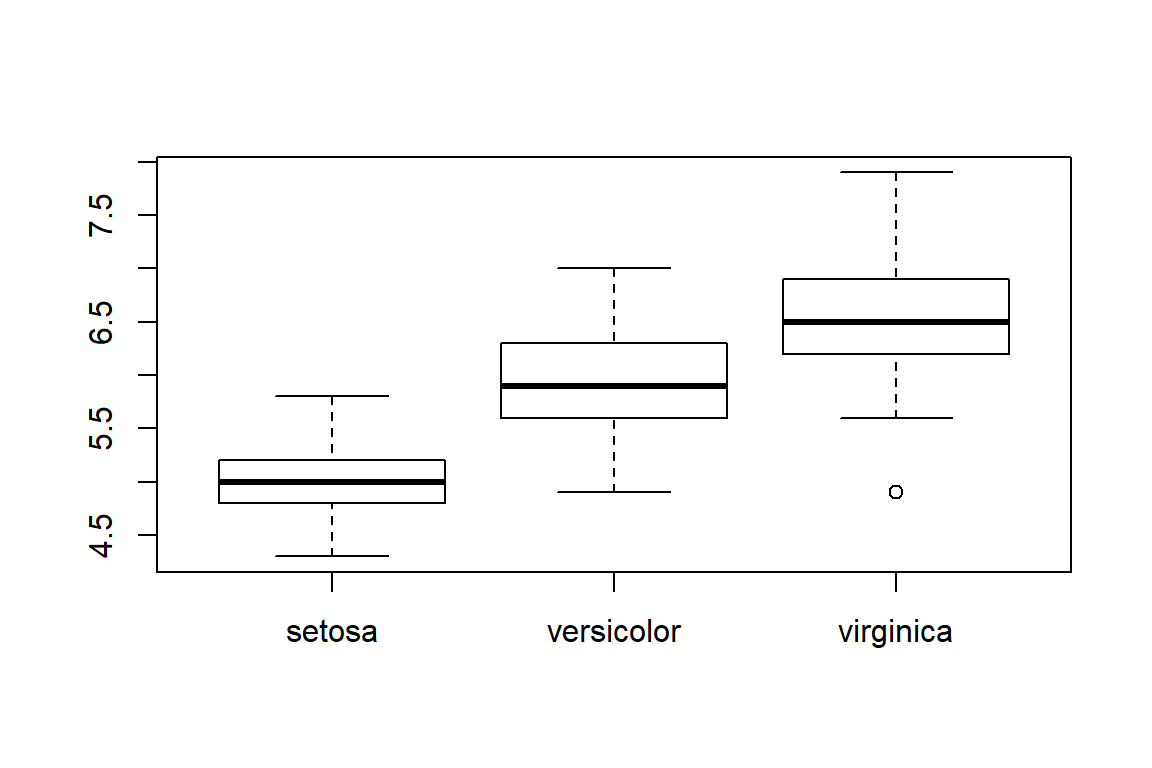
\includegraphics{IBSguide_files/figure-latex/unnamed-chunk-12-1.pdf}

What Motulsky shows in Figure 7.1 is sometimes now called a
\href{https://flowingdata.com/2016/09/08/beeswarm-plot-in-r-to-show-distributions/}{\textbf{beeswarm
plot}}, a name I like. They can be made in R using the
\href{http://www.cbs.dtu.dk/~eklund/beeswarm/}{beeswarm package}.

\begin{Shaded}
\begin{Highlighting}[]
\KeywordTok{beeswarm}\NormalTok{(Sepal.Length }\OperatorTok{~}\StringTok{ }\NormalTok{Species, }
         \DataTypeTok{data =}\NormalTok{ iris)}
\end{Highlighting}
\end{Shaded}

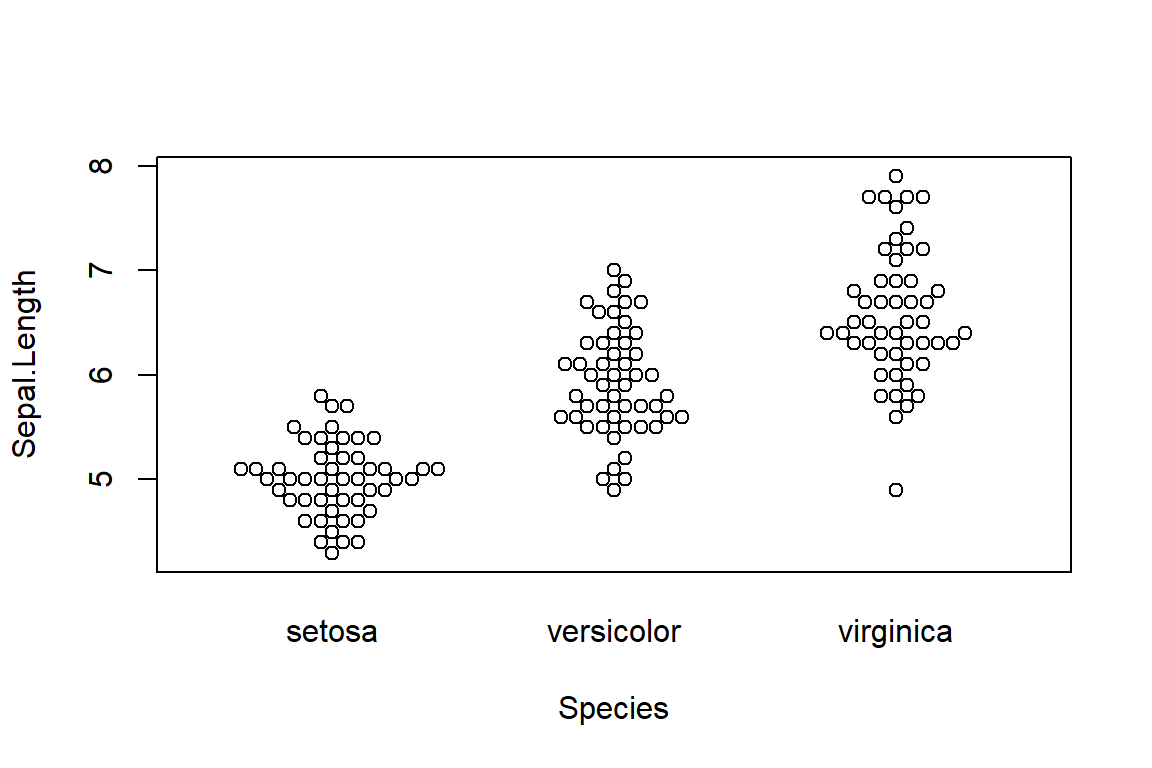
\includegraphics{IBSguide_files/figure-latex/unnamed-chunk-13-1.pdf}

A similar type of plot is a
\href{http://www.clayford.net/statistics/tag/strip-charts/}{stripchart}.
These work best when they are set up to not have their points
overlapping, which is called \textbf{jittering}.

\begin{Shaded}
\begin{Highlighting}[]
\KeywordTok{stripchart}\NormalTok{(Sepal.Length }\OperatorTok{~}\StringTok{ }\NormalTok{Species, }
           \DataTypeTok{data =}\NormalTok{ iris, }
           \DataTypeTok{vertical =} \OtherTok{TRUE}\NormalTok{, }
           \DataTypeTok{method=}\StringTok{"jitter"}\NormalTok{)}
\end{Highlighting}
\end{Shaded}

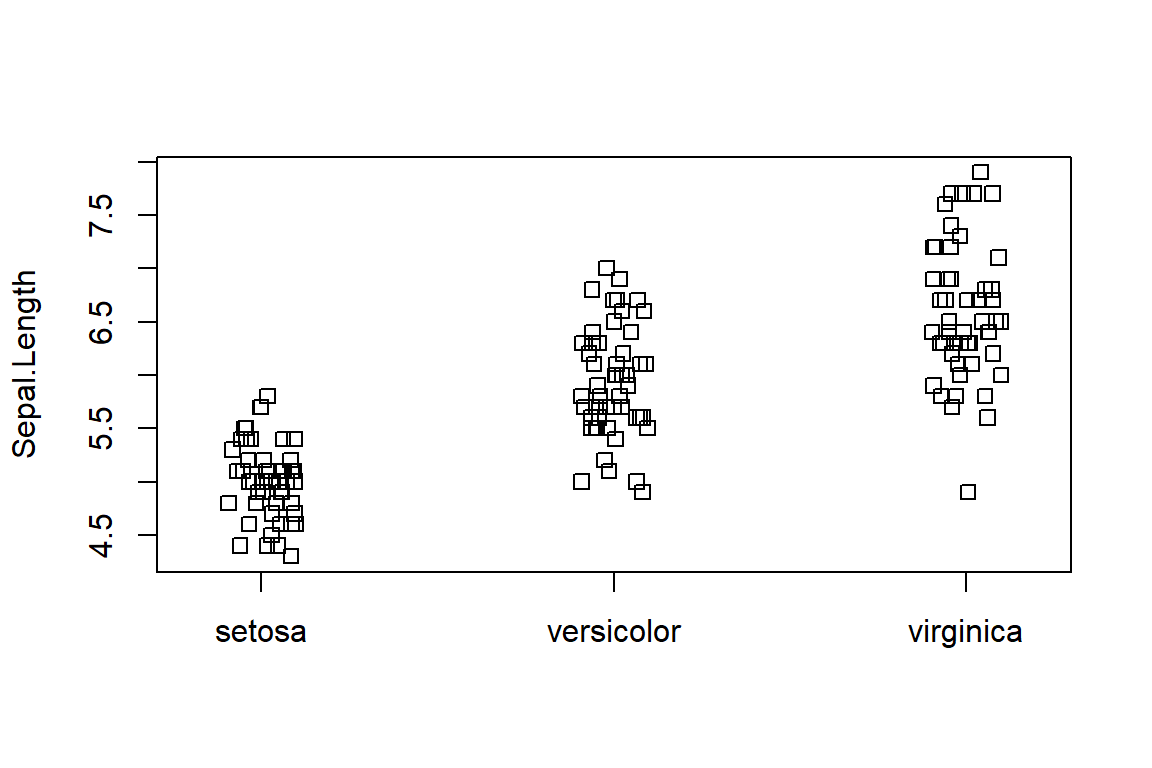
\includegraphics{IBSguide_files/figure-latex/unnamed-chunk-14-1.pdf}

A beeswarm plot is basically a jitter stripchart that has been well
organized. And has a cooler name.

\subsection{\texorpdfstring{``Box-and-whiskers
plots''}{Box-and-whiskers plots}}\label{box-and-whiskers-plots}

Usually just called a
\href{https://en.wikipedia.org/wiki/Box_plot}{\textbf{boxplot}}.

In base R they are made with the boxplot() command.

\begin{Shaded}
\begin{Highlighting}[]
\KeywordTok{boxplot}\NormalTok{(Sepal.Length }\OperatorTok{~}\StringTok{ }\NormalTok{Species, }
           \DataTypeTok{data =}\NormalTok{ iris, }
           \DataTypeTok{vertical =} \OtherTok{TRUE}\NormalTok{, }
           \DataTypeTok{method=}\StringTok{"jitter"}\NormalTok{)}
\end{Highlighting}
\end{Shaded}

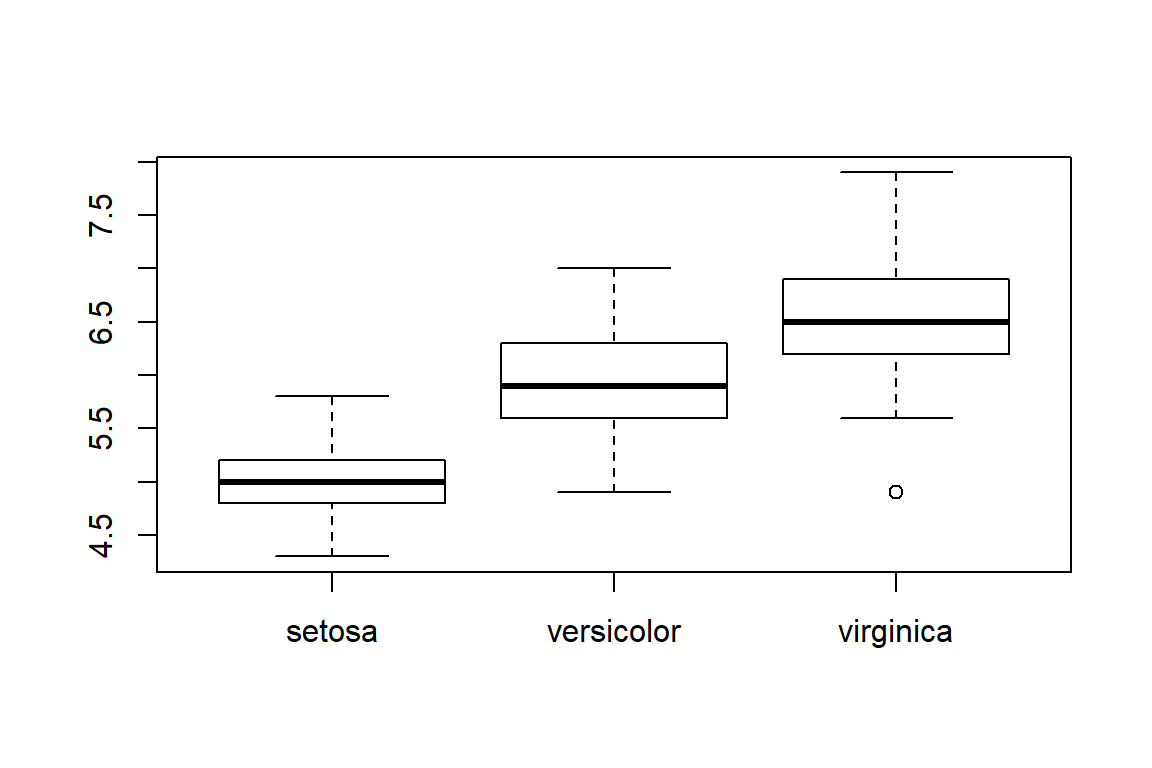
\includegraphics{IBSguide_files/figure-latex/unnamed-chunk-15-1.pdf}

In ggplot they can be made like this with the qplot() function

\begin{Shaded}
\begin{Highlighting}[]
\KeywordTok{qplot}\NormalTok{(}\DataTypeTok{data =}\NormalTok{ iris, }
      \DataTypeTok{y =}\NormalTok{ Sepal.Length,}
      \DataTypeTok{x =}\NormalTok{ Species,}
      \DataTypeTok{geom =} \StringTok{"boxplot"}\NormalTok{)}
\end{Highlighting}
\end{Shaded}

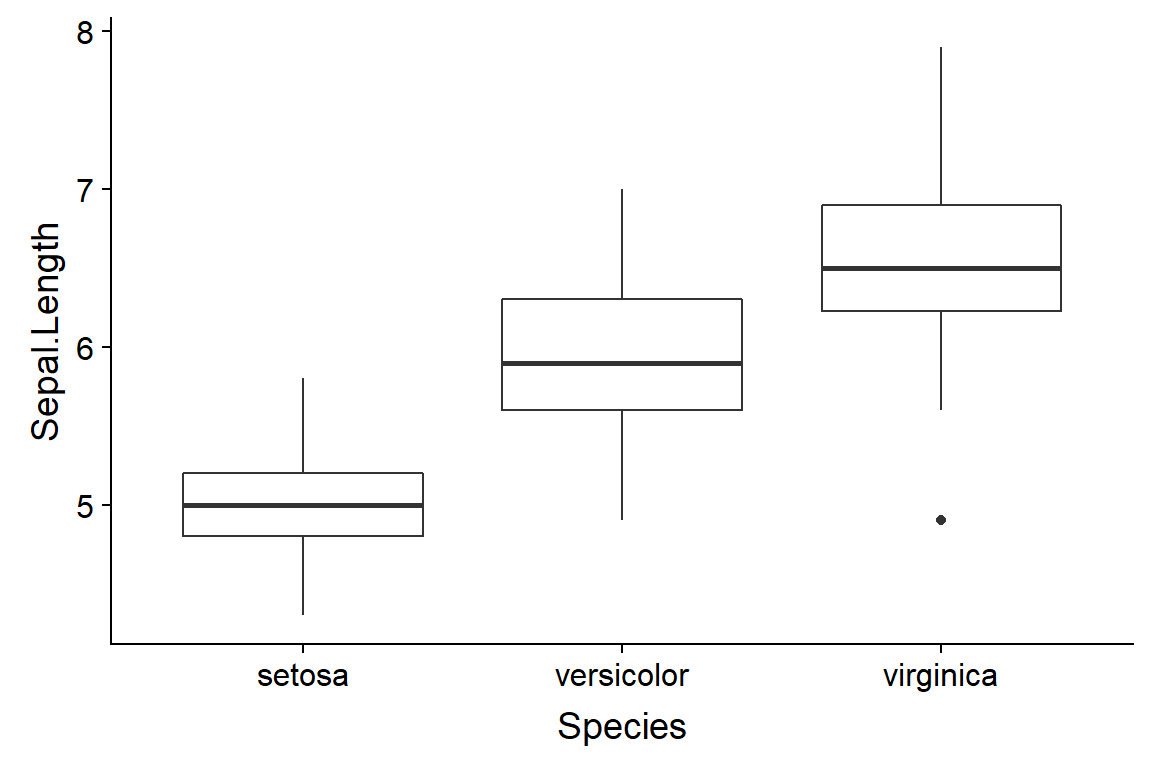
\includegraphics{IBSguide_files/figure-latex/unnamed-chunk-16-1.pdf}

Or directly with ggplot() using geom\_boxplot()

\begin{Shaded}
\begin{Highlighting}[]
\KeywordTok{ggplot}\NormalTok{(}\DataTypeTok{data =}\NormalTok{ iris,}
       \KeywordTok{aes}\NormalTok{(}\DataTypeTok{y =}\NormalTok{ Sepal.Length,}
           \DataTypeTok{x =}\NormalTok{ Species)) }\OperatorTok{+}
\StringTok{  }\KeywordTok{geom_boxplot}\NormalTok{()}
\end{Highlighting}
\end{Shaded}

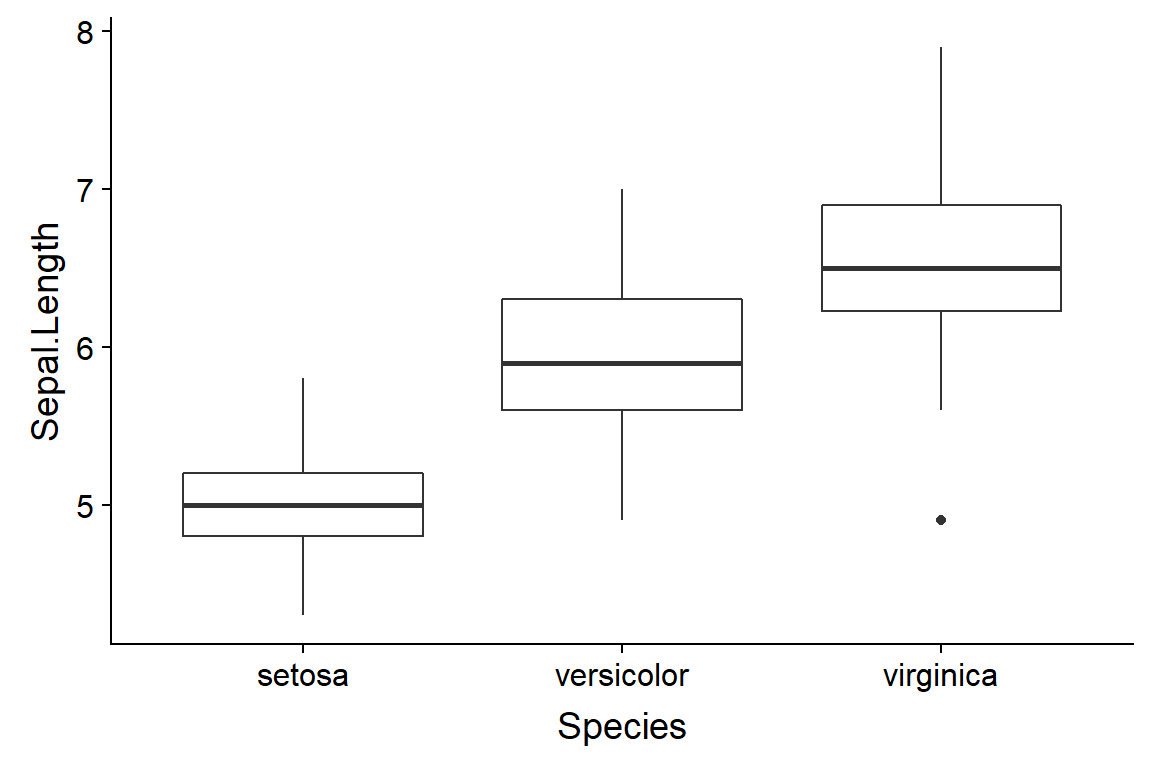
\includegraphics{IBSguide_files/figure-latex/unnamed-chunk-17-1.pdf}

\subsection{\texorpdfstring{``Violin
plots''}{Violin plots}}\label{violin-plots}

Violin plot can be useful when you want more information than given by a
boxplot but have too much data for a beeswarm. There's a package in R
which implements
\href{https://www.statmethods.net/graphs/boxplot.html}{violin plots} for
basic R graphics. In ggplot you use geom\_violin().

\begin{Shaded}
\begin{Highlighting}[]
\KeywordTok{ggplot}\NormalTok{(}\DataTypeTok{data =}\NormalTok{ iris,}
       \KeywordTok{aes}\NormalTok{(}\DataTypeTok{y =}\NormalTok{ Sepal.Length,}
           \DataTypeTok{x =}\NormalTok{ Species)) }\OperatorTok{+}
\StringTok{  }\KeywordTok{geom_violin}\NormalTok{()}
\end{Highlighting}
\end{Shaded}

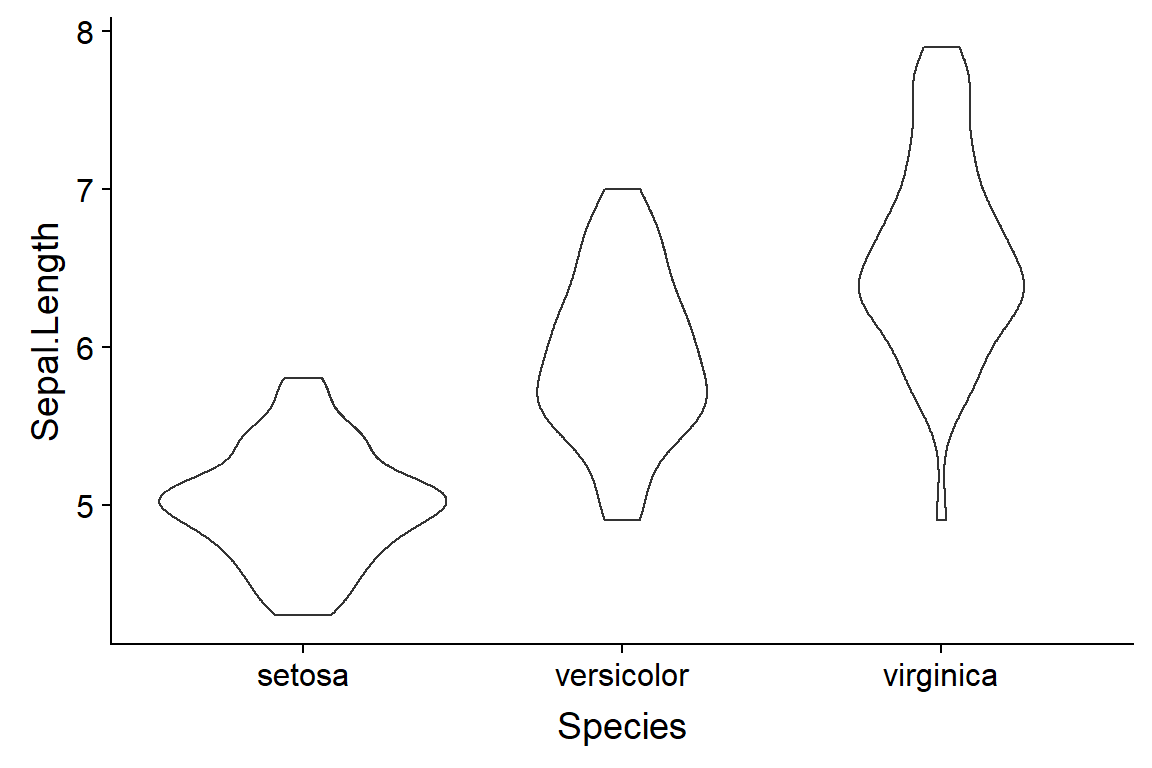
\includegraphics{IBSguide_files/figure-latex/unnamed-chunk-18-1.pdf}

\section{\texorpdfstring{``Graphing
Distributions''}{Graphing Distributions}}\label{graphing-distributions}

\subsection{\texorpdfstring{``Frequency
distributions''}{Frequency distributions}}\label{frequency-distributions}

\subsection{\texorpdfstring{``Cumulative frequency distribution''
(OPTIONAL)}{Cumulative frequency distribution (OPTIONAL)}}\label{cumulative-frequency-distribution-optional}

Good to know about but not applicable to most entry-level stats.

\section{\texorpdfstring{``Beware of Data
Massage''}{Beware of Data Massage}}\label{beware-of-data-massage}

\subsection{\texorpdfstring{``Beware of filtering out impossible
values''}{Beware of filtering out impossible values}}\label{beware-of-filtering-out-impossible-values}

\subsection{\texorpdfstring{``Beware of adjusting
data''}{Beware of adjusting data}}\label{beware-of-adjusting-data}

\subsection{\texorpdfstring{``Beware of
smoothing''}{Beware of smoothing}}\label{beware-of-smoothing}

\subsection{\texorpdfstring{``Beware of variable that are the ratio of
two
measurements''}{Beware of variable that are the ratio of two measurements}}\label{beware-of-variable-that-are-the-ratio-of-two-measurements}

\subsection{\texorpdfstring{``Beware of normalized
data''}{Beware of normalized data}}\label{beware-of-normalized-data}

\subsection*{Beware of ratios of
ratios}\label{beware-of-ratios-of-ratios}
\addcontentsline{toc}{subsection}{Beware of ratios of ratios}

Certo, et al. 2018. Divided We Fall: How Ratios Undermine Research in
Strategic Management
\url{http://journals.sagepub.com/doi/abs/10.1177/1094428118773455}

Curran-Everett, D. 2013. Explorations in statistics: the analysis of
ratios and normalized data.
\href{https://www.physiology.org/doi/abs/10.1152/advan.00053.2013}{Advances
in Physiology Education.}

Motulsky doesn't mention this. It can be a problem, though. Some papers
related to this topic:

Karp et al. 2012. The fallacy of ratio correction to address confounding
factors. Laboratory Animals 46: 245--252.

Koch et al. 2015. Overcoming problems with the use of ratios as
continuous characters for phylogenetic analyses. Zoologica Scripta.

\section{Q \& A}\label{q-a-1}

\section*{Further reading}\label{further-reading-5}
\addcontentsline{toc}{section}{Further reading}

\section*{References}\label{references-5}
\addcontentsline{toc}{section}{References}

\section*{Annotated Bibliography}\label{annotated-bibliography-2}
\addcontentsline{toc}{section}{Annotated Bibliography}

\chapter{\texorpdfstring{Chapter ``Types of
Variables''}{Chapter Types of Variables}}\label{chapter-types-of-variables}

\section*{Commentary}\label{commentary-6}
\addcontentsline{toc}{section}{Commentary}

\section*{Vocabulary}\label{vocabulary-7}
\addcontentsline{toc}{section}{Vocabulary}

\begin{itemize}
\tightlist
\item
  Binomial variable
\item
  Continous variable
\item
  Discrete varible
\item
  Interval variable
\item
  Nominal variable
\item
  ordinal variable
\item
  Ratio variable
\end{itemize}

\subsection{Motulsky vocab}\label{motulsky-vocab-7}

\subsection{Aditional vocab}\label{aditional-vocab-4}

\subsection{Key functions}\label{key-functions-6}

None

\section*{Chapter Notes}\label{chapter-notes-7}
\addcontentsline{toc}{section}{Chapter Notes}

\section{\texorpdfstring{``Continous
Variables''}{Continous Variables}}\label{continous-variables}

\subsection{\texorpdfstring{``Interval
variables''}{Interval variables}}\label{interval-variables}

\subsection{\texorpdfstring{``Ratio
variables''}{Ratio variables}}\label{ratio-variables}

\section{\texorpdfstring{``Discrete
Variables''}{Discrete Variables}}\label{discrete-variables}

\subsection{\texorpdfstring{``Ordinal
variables''}{Ordinal variables}}\label{ordinal-variables}

\subsection{\texorpdfstring{``Nominal and binomial
variables''}{Nominal and binomial variables}}\label{nominal-and-binomial-variables}

\section{\texorpdfstring{``Why It
Matters''}{Why It Matters}}\label{why-it-matters}

\section{\texorpdfstring{``Not Quite As Distinct As They
Seem''}{Not Quite As Distinct As They Seem}}\label{not-quite-as-distinct-as-they-seem}

\section{Q\&A}\label{qa}

\section*{Further reading}\label{further-reading-6}
\addcontentsline{toc}{section}{Further reading}

\section*{References}\label{references-6}
\addcontentsline{toc}{section}{References}

\section*{Annotated Bibliography}\label{annotated-bibliography-3}
\addcontentsline{toc}{section}{Annotated Bibliography}

\chapter{\texorpdfstring{Chapter ``Quantifying
Scatter''}{Chapter Quantifying Scatter}}\label{chapter-quantifying-scatter}

\section*{Commentary}\label{commentary-7}
\addcontentsline{toc}{section}{Commentary}

\section*{Vocabulary}\label{vocabulary-8}
\addcontentsline{toc}{section}{Vocabulary}

\subsection{Motulsky vocab}\label{motulsky-vocab-8}

\subsection{Aditional vocab}\label{aditional-vocab-5}

\subsection{Key functions}\label{key-functions-7}

None

\section*{Chapter Notes}\label{chapter-notes-8}
\addcontentsline{toc}{section}{Chapter Notes}

\section{\texorpdfstring{``Interpretting A Standard
Deviation''}{Interpretting A Standard Deviation}}\label{interpretting-a-standard-deviation}

\section{How It Works: Calculating
SD"}\label{how-it-works-calculating-sd}

\section{\texorpdfstring{``Why n-1?''}{Why n-1?}}\label{why-n-1}

\subsection{\texorpdfstring{``When it somes makes sense to use n in the
denominator''}{When it somes makes sense to use n in the denominator}}\label{when-it-somes-makes-sense-to-use-n-in-the-denominator}

\subsection{\texorpdfstring{``Why it usually makes sense to use n-1 in
the
denominator''}{Why it usually makes sense to use n-1 in the denominator}}\label{why-it-usually-makes-sense-to-use-n-1-in-the-denominator}

\subsection{\texorpdfstring{``The fine
print''}{The fine print}}\label{the-fine-print}

\section{\texorpdfstring{``Situations in Which n Can Seem
Ambiguous''}{Situations in Which n Can Seem Ambiguous}}\label{situations-in-which-n-can-seem-ambiguous}

\subsection{\texorpdfstring{``Replicate measurements within repae
experiments''}{Replicate measurements within repae experiments}}\label{replicate-measurements-within-repae-experiments}

\subsection{\texorpdfstring{``Eyes, ears and
elbos''}{Eyes, ears and elbos}}\label{eyes-ears-and-elbos}

\subsection{\texorpdfstring{``Representaitve
experiments''}{Representaitve experiments}}\label{representaitve-experiments}

\subsection{\texorpdfstring{``Trials with one
subject''}{Trials with one subject}}\label{trials-with-one-subject}

\section{\texorpdfstring{``SD and Sample
Size''}{SD and Sample Size}}\label{sd-and-sample-size}

\section{\texorpdfstring{``Other Ways to Quantify \& Display
Variability''}{Other Ways to Quantify \& Display Variability}}\label{other-ways-to-quantify-display-variability}

\subsection{\texorpdfstring{``Coefficient of
variation''}{Coefficient of variation}}\label{coefficient-of-variation}

\subsection{\texorpdfstring{``Variance''}{Variance}}\label{variance}

\subsection{\texorpdfstring{``Interquartile
range''}{Interquartile range}}\label{interquartile-range}

\subsection{\texorpdfstring{``Five-number
smmary''}{Five-number smmary}}\label{five-number-smmary}

\subsection{\texorpdfstring{``Median absolute
deviation''}{Median absolute deviation}}\label{median-absolute-deviation}

\section{Q\&A}\label{qa-1}

\section*{Further reading}\label{further-reading-7}
\addcontentsline{toc}{section}{Further reading}

\section*{References}\label{references-7}
\addcontentsline{toc}{section}{References}

\section*{Annotated Bibliography}\label{annotated-bibliography-4}
\addcontentsline{toc}{section}{Annotated Bibliography}

\chapter{\texorpdfstring{``The Gausian
Distribution''}{The Gausian Distribution}}\label{ch10}

\section*{Commentary}\label{commentary-8}
\addcontentsline{toc}{section}{Commentary}

\section*{Vocabulary}\label{vocabulary-9}
\addcontentsline{toc}{section}{Vocabulary}

\subsection*{Motulsky vocab}\label{motulsky-vocab-9}
\addcontentsline{toc}{subsection}{Motulsky vocab}

\subsection*{Aditional vocab}\label{aditional-vocab-6}
\addcontentsline{toc}{subsection}{Aditional vocab}

\section*{Key functions}\label{key-functions-8}
\addcontentsline{toc}{section}{Key functions}

None

\section*{Chapter Notes}\label{chapter-notes-9}
\addcontentsline{toc}{section}{Chapter Notes}

\section{\texorpdfstring{{[} {]} ``''}{{[} {]} }}\label{section-9}

\section{\texorpdfstring{{[} {]} ``''}{{[} {]} }}\label{section-10}

\section{\texorpdfstring{{[} {]} ``''}{{[} {]} }}\label{section-11}

\section*{Further reading}\label{further-reading-8}
\addcontentsline{toc}{section}{Further reading}

\section*{References}\label{references-8}
\addcontentsline{toc}{section}{References}

\chapter{\texorpdfstring{``The Lognormal Distribution and Geometric
Mean''}{The Lognormal Distribution and Geometric Mean}}\label{ch11}

\section*{Commentary}\label{commentary-9}
\addcontentsline{toc}{section}{Commentary}

\section*{Vocabulary}\label{vocabulary-10}
\addcontentsline{toc}{section}{Vocabulary}

\subsection*{Motulsky vocab}\label{motulsky-vocab-10}
\addcontentsline{toc}{subsection}{Motulsky vocab}

\subsection*{Aditional vocab}\label{aditional-vocab-7}
\addcontentsline{toc}{subsection}{Aditional vocab}

\section*{Key functions}\label{key-functions-9}
\addcontentsline{toc}{section}{Key functions}

None

\section*{Chapter Notes}\label{chapter-notes-10}
\addcontentsline{toc}{section}{Chapter Notes}

\section{\texorpdfstring{{[} {]} ``''}{{[} {]} }}\label{section-12}

\section{\texorpdfstring{{[} {]} ``''}{{[} {]} }}\label{section-13}

\section{\texorpdfstring{{[} {]} ``''}{{[} {]} }}\label{section-14}

\section*{Further reading}\label{further-reading-9}
\addcontentsline{toc}{section}{Further reading}

\section*{References}\label{references-9}
\addcontentsline{toc}{section}{References}

\chapter{\texorpdfstring{``Confidence Interval of a
Mean''}{Confidence Interval of a Mean}}\label{ch12}

\section*{Commentary}\label{commentary-10}
\addcontentsline{toc}{section}{Commentary}

\section*{Vocabulary}\label{vocabulary-11}
\addcontentsline{toc}{section}{Vocabulary}

\subsection*{Motulsky vocab}\label{motulsky-vocab-11}
\addcontentsline{toc}{subsection}{Motulsky vocab}

\subsection*{Aditional vocab}\label{aditional-vocab-8}
\addcontentsline{toc}{subsection}{Aditional vocab}

\section*{Key functions}\label{key-functions-10}
\addcontentsline{toc}{section}{Key functions}

None

\section*{Chapter Notes}\label{chapter-notes-11}
\addcontentsline{toc}{section}{Chapter Notes}

\section{\texorpdfstring{{[} {]} ``''}{{[} {]} }}\label{section-15}

\section{\texorpdfstring{{[} {]} ``''}{{[} {]} }}\label{section-16}

\section{\texorpdfstring{{[} {]} ``''}{{[} {]} }}\label{section-17}

\section*{Further reading}\label{further-reading-10}
\addcontentsline{toc}{section}{Further reading}

\section*{References}\label{references-10}
\addcontentsline{toc}{section}{References}

\chapter{\texorpdfstring{``The Theory of Confidence
Intervals''}{The Theory of Confidence Intervals}}\label{ch13}

\section*{Commentary}\label{commentary-11}
\addcontentsline{toc}{section}{Commentary}

\section*{Vocabulary}\label{vocabulary-12}
\addcontentsline{toc}{section}{Vocabulary}

\subsection*{Motulsky vocab}\label{motulsky-vocab-12}
\addcontentsline{toc}{subsection}{Motulsky vocab}

\subsection*{Aditional vocab}\label{aditional-vocab-9}
\addcontentsline{toc}{subsection}{Aditional vocab}

\section*{Key functions}\label{key-functions-11}
\addcontentsline{toc}{section}{Key functions}

None

\section*{Chapter Notes}\label{chapter-notes-12}
\addcontentsline{toc}{section}{Chapter Notes}

\section{\texorpdfstring{{[} {]} ``''}{{[} {]} }}\label{section-18}

\section{\texorpdfstring{{[} {]} ``''}{{[} {]} }}\label{section-19}

\section{\texorpdfstring{{[} {]} ``''}{{[} {]} }}\label{section-20}

\section*{Further reading}\label{further-reading-11}
\addcontentsline{toc}{section}{Further reading}

\section*{References}\label{references-11}
\addcontentsline{toc}{section}{References}

\begin{verbatim}
## 
## Attaching package: 'zoo'
\end{verbatim}

\begin{verbatim}
## The following objects are masked from 'package:base':
## 
##     as.Date, as.Date.numeric
\end{verbatim}

\chapter{\texorpdfstring{``Error Bars''}{Error Bars}}\label{error-bars}

\section*{Commentary}\label{commentary-12}
\addcontentsline{toc}{section}{Commentary}

\begin{quote}
``\ldots{}the standard deviation is a measure of the variability of a
set of observations, whereas the standard error is a measure of the
precision of an estimate\ldots{}in relation to its unknown true value.''
(Altman 1980 ``Statistics and ethics in medical research VI:
Presentation of results''. BMJ)
\end{quote}

\section*{Vocabulary}\label{vocabulary-13}
\addcontentsline{toc}{section}{Vocabulary}

\subsection*{Motulsky vocab}\label{motulsky-vocab-13}
\addcontentsline{toc}{subsection}{Motulsky vocab}

\subsection*{Aditional vocab}\label{aditional-vocab-10}
\addcontentsline{toc}{subsection}{Aditional vocab}

\subsection*{Key functions}\label{key-functions-12}
\addcontentsline{toc}{subsection}{Key functions}

\section*{Chapter Notes}\label{chapter-notes-13}
\addcontentsline{toc}{section}{Chapter Notes}

\section{\texorpdfstring{{[} {]} ``SD VERSUS
SEM''}{{[} {]} SD VERSUS SEM}}\label{sd-versus-sem}

\subsection{\texorpdfstring{{[} {]} ``What is the
SD''}{{[} {]} What is the SD}}\label{what-is-the-sd}

{[} {]} The \textbf{standard deviation} is a measure of variability. The
larger the standard deviation is, the more variation there is within a
sample. When variation is large within a \textbf{sample}, its likely
that there is lots of variation within the \textbf{population} that was
sampled. The standard deviation does not directly inform your opinion
about the \textbf{sample mean.}

\subsubsection*{The SD in Excel}\label{the-sd-in-excel}
\addcontentsline{toc}{subsubsection}{The SD in Excel}

In Excel they distinquish between the population standard deviation,
STDEV.P(), and the \textbf{sample standard deviation}, STDEV.S(). In
practice you almost never are working with a population.

\subsubsection*{The SD in R}\label{the-sd-in-r}
\addcontentsline{toc}{subsubsection}{The SD in R}

The standard deviation is calcualted in R using the function sd()

\begin{Shaded}
\begin{Highlighting}[]
\NormalTok{some.data <-}\StringTok{ }\KeywordTok{c}\NormalTok{(}\DecValTok{1}\NormalTok{,}\DecValTok{4}\NormalTok{,}\DecValTok{5}\NormalTok{,}\DecValTok{6}\NormalTok{)}
\KeywordTok{sd}\NormalTok{(some.data)}
\end{Highlighting}
\end{Shaded}

\begin{verbatim}
## [1] 2.160247
\end{verbatim}

The standard deviation is the square root of the variance.

\begin{Shaded}
\begin{Highlighting}[]
\CommentTok{# the variance of some.data}
\KeywordTok{var}\NormalTok{(some.data)}
\end{Highlighting}
\end{Shaded}

\begin{verbatim}
## [1] 4.666667
\end{verbatim}

\begin{Shaded}
\begin{Highlighting}[]
\CommentTok{#square root of the variance of some.data}
\KeywordTok{sqrt}\NormalTok{(}\KeywordTok{var}\NormalTok{(some.data))}
\end{Highlighting}
\end{Shaded}

\begin{verbatim}
## [1] 2.160247
\end{verbatim}

\begin{Shaded}
\begin{Highlighting}[]
\CommentTok{#the standard deviation = the square root of the variance}
\KeywordTok{sd}\NormalTok{(some.data) }\OperatorTok{==}\StringTok{ }\KeywordTok{sqrt}\NormalTok{(}\KeywordTok{var}\NormalTok{(some.data))}
\end{Highlighting}
\end{Shaded}

\begin{verbatim}
## [1] TRUE
\end{verbatim}

\subsection{\texorpdfstring{{[} {]} ``What is the
SEM?''}{{[} {]} What is the SEM?}}\label{what-is-the-sem}

\subsection{\texorpdfstring{{[} {]} ``The SEM does not quanitfy
variablity among
variables''}{{[} {]} The SEM does not quanitfy variablity among variables}}\label{the-sem-does-not-quanitfy-variablity-among-variables}

\subsection{\texorpdfstring{{[} {]} ``The SEM quantifies how precisely
you know the population
mean''}{{[} {]} The SEM quantifies how precisely you know the population mean}}\label{the-sem-quantifies-how-precisely-you-know-the-population-mean}

{[} {]} Challenge question: how would you describe the difference
between the \textbf{population mean} and the \textbf{same mean?}

\subsubsection*{{[} {]} SEM Summary}\label{sem-summary}
\addcontentsline{toc}{subsubsection}{{[} {]} SEM Summary}

\begin{quote}
``The standard deviation (often SD) is a measure of variability. When we
calculate the standard deviation of a sample, we are using it as an
estimate of the variability of the population from which the sample was
drawn \ldots{} So, if we want to say how widely scattered some
measurements are, we use the standard deviation. If we want to indicate
the uncertainty around the estimate of the mean measurement, we quote
the standard error of the mean.'' Altman (2013)
\end{quote}

\textbf{standard error of the mean (SEM)} or just \textbf{standard error
(SE)} is a measure of \textbf{precision.} The \textbf{standard error
does not tell you anything about variation in your sample or the
population.} The standard error tells you about how precisely you have
estimated your mean (Note that standard errors can also be calcualted
for other things.) A large standard error means the mean has been
estimately with low precision. A small standard error means that the
mean has been estimate precisely. Precision is increased by either
little variation in the population or a larger sample size.

\subsection{\texorpdfstring{{[} {]} ``How to compute the SD from the
SEM''}{{[} {]} How to compute the SD from the SEM}}\label{how-to-compute-the-sd-from-the-sem}

If you are given a SEM and sample size, you can \textbf{back calculate}
the standard deviation. You should always make your same size clear for
your statistical tests (or, equivalently, the \textbf{degrees of
freedom}, which we'll talk about later) so people can calculate the SD
if they want it.

\section{\texorpdfstring{{[} {]} ``WHICH KIND OF ERROR BAR SHOULD I
PLOT''}{{[} {]} WHICH KIND OF ERROR BAR SHOULD I PLOT}}\label{which-kind-of-error-bar-should-i-plot}

\subsection{\texorpdfstring{{[} {]} ``Goal: To Show the variation among
the
values''}{{[} {]} Goal: To Show the variation among the values}}\label{goal-to-show-the-variation-among-the-values}

\subsection{\texorpdfstring{{[} {]} ``Goal: To show how precisely you
have determined the population
mean''}{{[} {]} Goal: To show how precisely you have determined the population mean}}\label{goal-to-show-how-precisely-you-have-determined-the-population-mean}

{[} {]} If this is your goal, you should just plot the 95\% CI. Or
better yet, plot both! I like plots like this

\begin{verbatim}
## 
## Attaching package: 'coefplot'
\end{verbatim}

\begin{verbatim}
## The following objects are masked from 'package:arm':
## 
##     coefplot, coefplot.default, invlogit
\end{verbatim}

\begin{verbatim}
## Warning: Removed 1 rows containing missing values (geom_vline).
\end{verbatim}

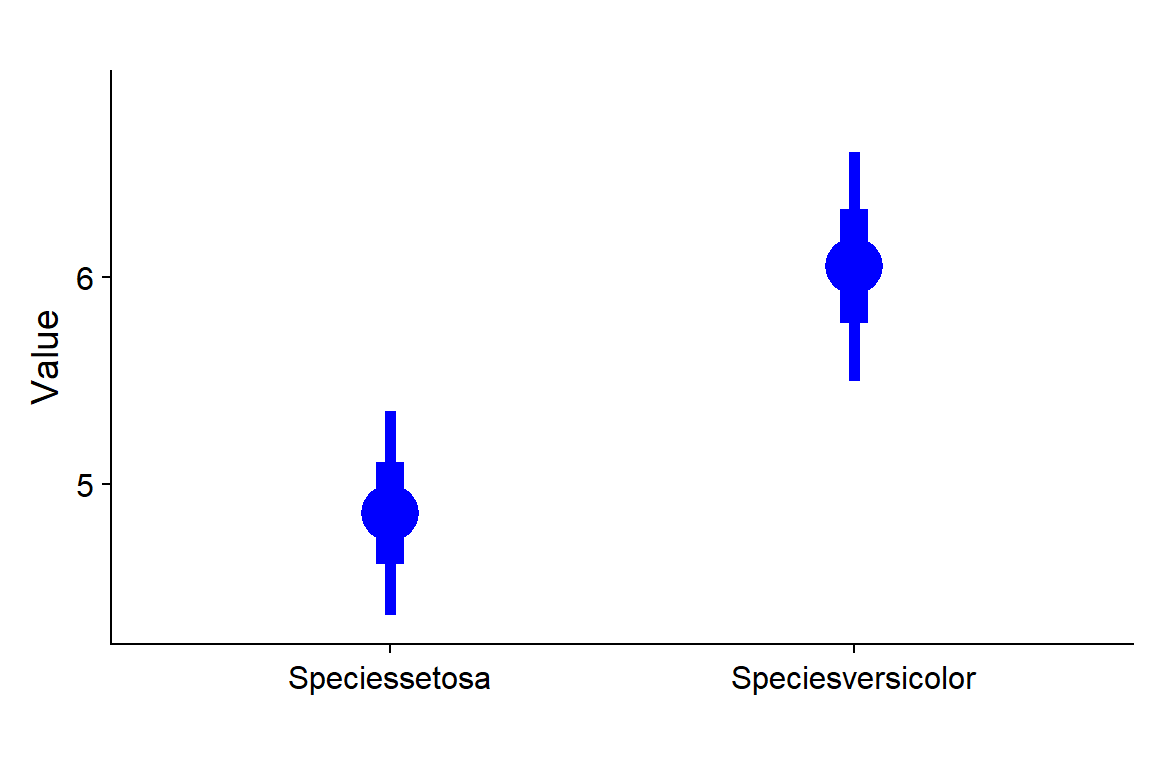
\includegraphics{IBSguide_files/figure-latex/unnamed-chunk-26-1.pdf}

\subsection{\texorpdfstring{{[} {]} ``Goal: To create persuaive
propaganda''}{{[} {]} Goal: To create persuaive propaganda}}\label{goal-to-create-persuaive-propaganda}

``Because they are shorter than the 95\% CI'' is \emph{not} a good
reason to use SEM.

\section{\texorpdfstring{{[} {]} ``THE APPEARANCE OF ERROR
BARS''}{{[} {]} THE APPEARANCE OF ERROR BARS}}\label{the-appearance-of-error-bars}

I personally don't like bar plots (eg right side of figure 14.1 on page
121) and see no reason not to just use a dot with error bars for the
mean, and to include the raw data whenever possible.

For a middle of the road opinion on bar plot see Ben Bolker: ``Dynamite
plots: unmitigated evil?''
\url{http://emdbolker.wikidot.com/blog:dynamite}

For people who realy don't like them
\url{http://biostat.mc.vanderbilt.edu/wiki/Main/DynamitePlots}

I think this sums up one of the main reasons barplots are bad: ``bar
graphs that boil down data points to a single mean often fail to convey
the nuances of the numbers''
\url{https://www.nature.com/news/bar-graphs-criticized-for-misrepresenting-data-1.17383}

I really don't like barplots that only include the upper error bar (as
in figure 14.2). I see no reason why you should do this.

\section{\texorpdfstring{{[}!{]} ``HOW ARE SD AND SEM RELATED TO SAMPLE
SIZE''"}{{[}!{]} HOW ARE SD AND SEM RELATED TO SAMPLE SIZE"}}\label{how-are-sd-and-sem-related-to-sample-size}

\subsection{\texorpdfstring{{[} {]} ``If you increase the sample size,
is the SEM expected to get larger, get smaller, or stay about the
same?''}{{[} {]} If you increase the sample size, is the SEM expected to get larger, get smaller, or stay about the same?}}\label{if-you-increase-the-sample-size-is-the-sem-expected-to-get-larger-get-smaller-or-stay-about-the-same}

{[} {]} This would make a great test question.

\subsection{\texorpdfstring{{[} {]} ``If you increase the sample size,
is the SD expected to get larger, get smaller, or stay about the
same?''}{{[} {]} If you increase the sample size, is the SD expected to get larger, get smaller, or stay about the same?}}\label{if-you-increase-the-sample-size-is-the-sd-expected-to-get-larger-get-smaller-or-stay-about-the-same}

{[} {]} This would make a great test question.

\subsubsection{Simulating SEM/SD changes with sample
size}\label{simulating-semsd-changes-with-sample-size}

The mean and SD look like this
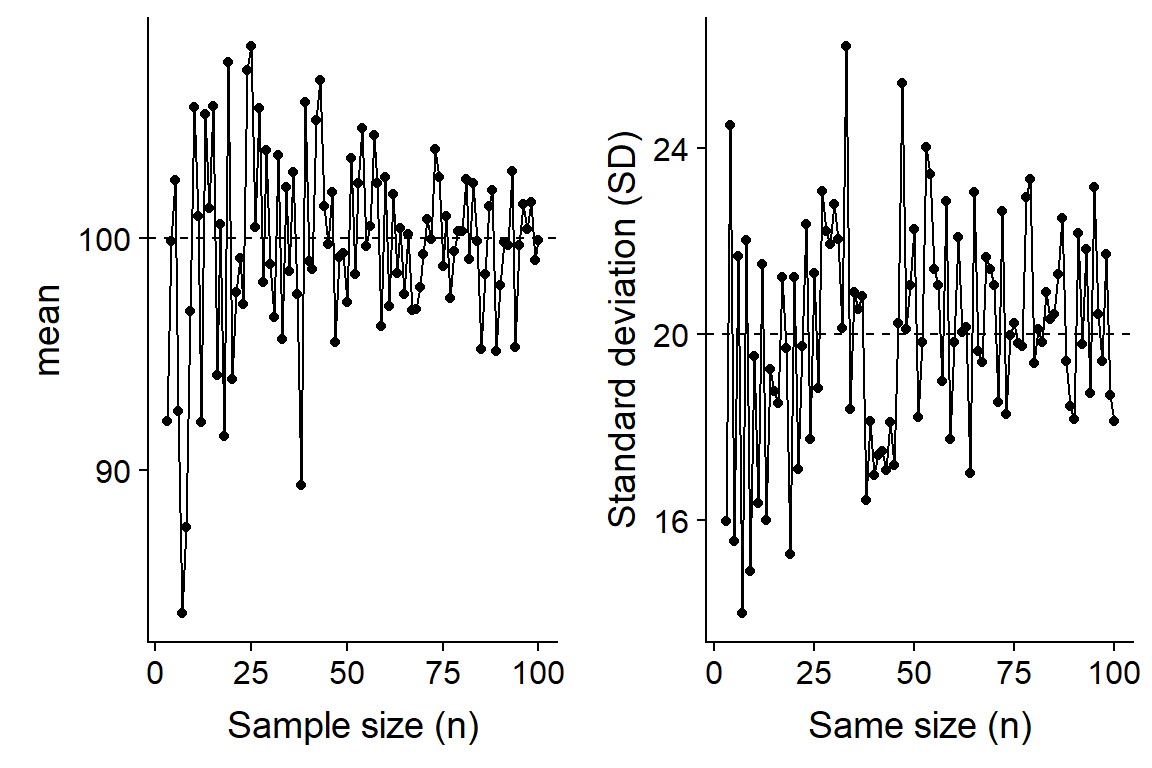
\includegraphics{IBSguide_files/figure-latex/unnamed-chunk-28-1.pdf}

The SE looks like this
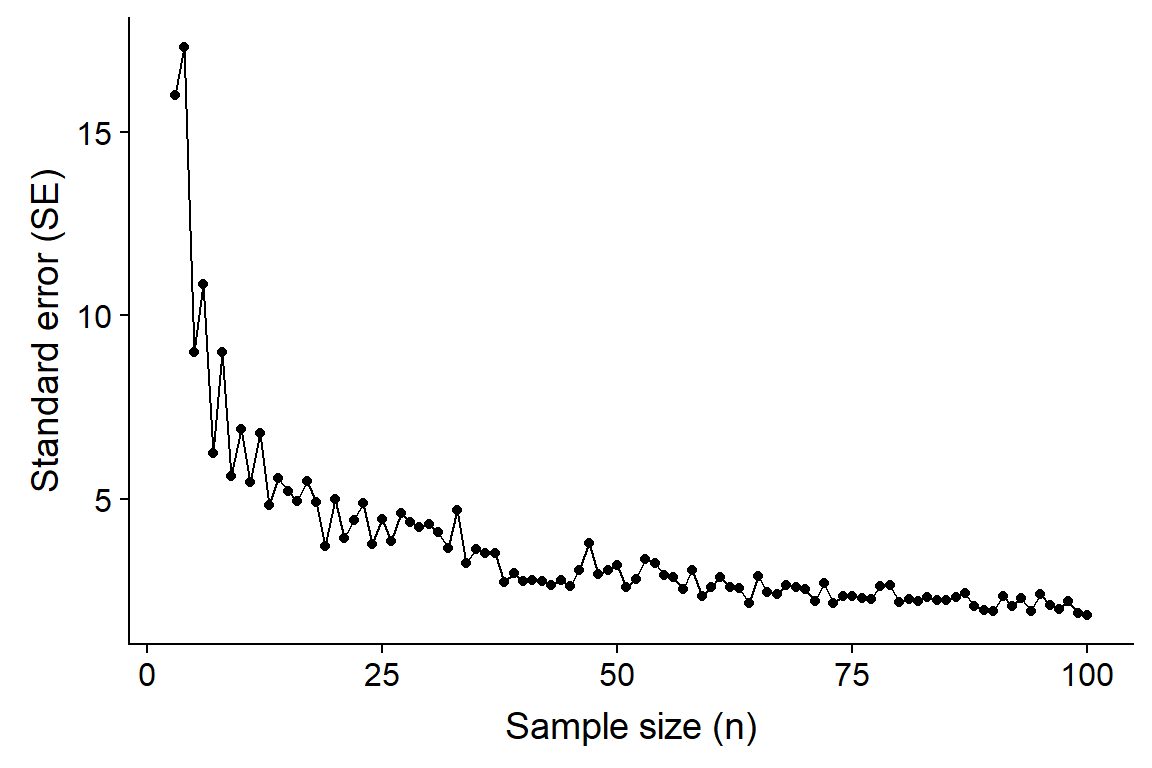
\includegraphics{IBSguide_files/figure-latex/unnamed-chunk-29-1.pdf}

\section{\texorpdfstring{``GEOMETRIC SD ERROR BARS''
(SKIP)}{GEOMETRIC SD ERROR BARS (SKIP)}}\label{geometric-sd-error-bars-skip}

\section{\texorpdfstring{{[} {]} ``COMMON MISTAKES: ERROR
BARS''}{{[} {]} COMMON MISTAKES: ERROR BARS}}\label{common-mistakes-error-bars}

\subsection{\texorpdfstring{{[} {]} ``Mistake: Plotting mean \& error
bar instead of plotting a frequency
distribution''}{{[} {]} Mistake: Plotting mean \& error bar instead of plotting a frequency distribution}}\label{mistake-plotting-mean-error-bar-instead-of-plotting-a-frequency-distribution}

For more on this see Weissgerber. 2015. Beyond Bar and Line Graphs: Time
for a New Data Presentation Paradigm. PLoS.
\url{http://journals.plos.org/plosbiology/article?id=10.1371/journal.pbio.1002128\&fullSite}

\subsection{\texorpdfstring{{[} {]} ``Mistake: Assuming that all
distributions are
Gaussian''}{{[} {]} Mistake: Assuming that all distributions are Gaussian}}\label{mistake-assuming-that-all-distributions-are-gaussian}

Pop quiz: \textbf{Gaussian} is the same as
\_\_\_\_\_\_\_\_\_\_\_\_\_\_\_\_\_\_

\subsection{\texorpdfstring{{[} {]} ``Mistake: Plotting a mean \& error
bar w/o defining how the error bars were
computed.''}{{[} {]} Mistake: Plotting a mean \& error bar w/o defining how the error bars were computed.}}\label{mistake-plotting-a-mean-error-bar-wo-defining-how-the-error-bars-were-computed.}

A figure legend should always state what the error bars are. Even
better, put an annotation within the plot itself.

\section{{[} {]} Q\&A}\label{qa-2}

\section*{Further reading}\label{further-reading-12}
\addcontentsline{toc}{section}{Further reading}

The difference between SD and SEM are a perrenial topic. If things are
clear check out one of these resources. Better yet, print one out an
post in on your lab bulletin board - chances are other people are fuzzy
on it too!

``Standard deviation versus standard error''
\url{http://thestatsgeek.com/2013/06/30/standard-deviation-versus-standard-error/}

``Basic stats:Standard deviation vs Standard error''
\url{https://datascienceplus.com/standard-deviation-vs-standard-error/}

Altman 2005. Standard deviations and standard errors BMJ 331 doi:
\url{https://doi.org/10.1136/bmj.331.7521.903} (Published 13 October
2005)

Klaus 2015. Statistical relevance---relevant statistics, part II:
presenting experimental data. EMBO Journal.
\url{http://emboj.embopress.org/content/early/2016/07/18/embj.201694659?casa_token=h0I6nRzyLsYAAAAA\%3AvvaeRts7NpFZwgiDctKC7z0qbvvd7OTJ1d-XgsW1mvg7BJPpOvVnTuwGNjLP0r1DWvbVJ9gGfkfqg6I}

Cummings et al. 2007.\\
Error bars in experimental biology. Journal of Cell Biology.
\url{http://jcb.rupress.org/content/177/1/7.short}

Munger 2007. Most researchers don't understand error bars. Cognitive
Daily.
\url{http://scienceblogs.com/cognitivedaily/2007/03/29/most-researchers-dont-understa/}

Wullschleger et al. 2014. High Incorrect Use of the Standard Error of
the Mean (SEM) in Original Articles in Three Cardiovascular Journals
Evaluated for 2012. PLoS BIology.
\url{http://journals.plos.org/plosone/article?id=10.1371/journal.pone.0110364}

\section*{References}\label{references-12}
\addcontentsline{toc}{section}{References}

\section*{Annotated Bibliography}\label{annotated-bibliography-5}
\addcontentsline{toc}{section}{Annotated Bibliography}

\chapter{\texorpdfstring{``Introducing
P-Values''}{Introducing P-Values}}\label{ch15}

\section*{Commentary}\label{commentary-13}
\addcontentsline{toc}{section}{Commentary}

\section*{Vocabulary}\label{vocabulary-14}
\addcontentsline{toc}{section}{Vocabulary}

\subsection*{Motulsky vocab}\label{motulsky-vocab-14}
\addcontentsline{toc}{subsection}{Motulsky vocab}

\subsection*{Aditional vocab}\label{aditional-vocab-11}
\addcontentsline{toc}{subsection}{Aditional vocab}

\section*{Key functions}\label{key-functions-13}
\addcontentsline{toc}{section}{Key functions}

None

\section*{Chapter Notes}\label{chapter-notes-14}
\addcontentsline{toc}{section}{Chapter Notes}

\section{\texorpdfstring{{[} {]} ``''}{{[} {]} }}\label{section-21}

\section{\texorpdfstring{{[} {]} ``''}{{[} {]} }}\label{section-22}

\section{\texorpdfstring{{[} {]} ``''}{{[} {]} }}\label{section-23}

\section*{Further reading}\label{further-reading-13}
\addcontentsline{toc}{section}{Further reading}

\section*{References}\label{references-13}
\addcontentsline{toc}{section}{References}

\chapter{\texorpdfstring{``Statistical Significance and Hypothesis
Testing''}{Statistical Significance and Hypothesis Testing}}\label{ch16}

\section*{Commentary}\label{commentary-14}
\addcontentsline{toc}{section}{Commentary}

\section*{Vocabulary}\label{vocabulary-15}
\addcontentsline{toc}{section}{Vocabulary}

\subsection*{Motulsky vocab}\label{motulsky-vocab-15}
\addcontentsline{toc}{subsection}{Motulsky vocab}

\subsection*{Aditional vocab}\label{aditional-vocab-12}
\addcontentsline{toc}{subsection}{Aditional vocab}

\section*{Key functions}\label{key-functions-14}
\addcontentsline{toc}{section}{Key functions}

None

\section*{Chapter Notes}\label{chapter-notes-15}
\addcontentsline{toc}{section}{Chapter Notes}

\section{\texorpdfstring{{[} {]} ``''}{{[} {]} }}\label{section-24}

\section{\texorpdfstring{{[} {]} ``''}{{[} {]} }}\label{section-25}

\section{\texorpdfstring{{[} {]} ``''}{{[} {]} }}\label{section-26}

\section*{Further reading}\label{further-reading-14}
\addcontentsline{toc}{section}{Further reading}

\section*{References}\label{references-14}
\addcontentsline{toc}{section}{References}

\chapter{\texorpdfstring{``COmparing Groups with Confidence Intervals
and P
Values''}{COmparing Groups with Confidence Intervals and P Values}}\label{ch17}

\section*{Commentary}\label{commentary-15}
\addcontentsline{toc}{section}{Commentary}

\section*{Vocabulary}\label{vocabulary-16}
\addcontentsline{toc}{section}{Vocabulary}

\subsection*{Motulsky vocab}\label{motulsky-vocab-16}
\addcontentsline{toc}{subsection}{Motulsky vocab}

\subsection*{Aditional vocab}\label{aditional-vocab-13}
\addcontentsline{toc}{subsection}{Aditional vocab}

\section*{Key functions}\label{key-functions-15}
\addcontentsline{toc}{section}{Key functions}

None

\section*{Chapter Notes}\label{chapter-notes-16}
\addcontentsline{toc}{section}{Chapter Notes}

\section{\texorpdfstring{{[} {]} ``''}{{[} {]} }}\label{section-27}

\section{\texorpdfstring{{[} {]} ``''}{{[} {]} }}\label{section-28}

\section{\texorpdfstring{{[} {]} ``''}{{[} {]} }}\label{section-29}

\section*{Further reading}\label{further-reading-15}
\addcontentsline{toc}{section}{Further reading}

\section*{References}\label{references-15}
\addcontentsline{toc}{section}{References}

\bibliography{book.bib}


\end{document}
